\documentclass{article}

% If your paper is accepted, change the options for the package
% aistats2020 as follows:
%
% \usepackage[accepted]{aistats2020}
%
% This option will print headings for the title of your paper and
% headings for the authors names, plus a copyright note at the end of
% the first column of the first page.

% If you set papersize explicitly, activate the following three lines:
%\special{papersize = 8.5in, 11in}
%\setlength{\pdfpageheight}{11in}
%\setlength{\pdfpagewidth}{8.5in}

% If you use natbib package, activate the following three lines:
\usepackage[round]{natbib}
\renewcommand{\bibname}{References}
\renewcommand{\bibsection}{\subsubsection*{\bibname}}

% If you use BibTeX in apalike style, activate the following line:
%\bibliographystyle{apalike}

\usepackage[utf8]{inputenc} % allow utf-8 input
\usepackage[T1]{fontenc}    % use 8-bit T1 fonts
\usepackage{hyperref}       % hyperlinks
\usepackage{url}            % simple URL typesetting
\usepackage{booktabs}       % professional-quality tables
\usepackage{amsfonts}       % blackboard math symbols
\usepackage{nicefrac}       % compact symbols for 1/2, etc.
\usepackage{microtype}      % microtypography

% My packages

\usepackage[mathscr]{euscript}
\usepackage{graphicx}
\usepackage {tikz}
\usetikzlibrary {positioning}
\usetikzlibrary{shapes.misc}
\usetikzlibrary{shapes.geometric}
\usetikzlibrary{calc}
\usetikzlibrary{arrows.meta}
\usepackage{amsthm}
\usepackage{amsmath}
\usepackage{amssymb}
\usepackage{dsfont}
\usepackage{stmaryrd }
\usepackage{csquotes}
\usepackage{wasysym}
\usepackage[]{todonotes}

 
\theoremstyle{remark}
\newtheorem*{remark}{Remark}

\theoremstyle{plain}
\newtheorem{theorem}{Theorem}[section]
\newtheorem{corollary}[theorem]{Corollary}
\newtheorem{lemma}[theorem]{Lemma}
\newtheorem{proposition}[theorem]{Proposition}


\newtheorem{innercustomthm}{Theorem}
\newenvironment{customthm}[1]
  {\renewcommand\theinnercustomthm{#1}\innercustomthm}
  {\endinnercustomthm}

\theoremstyle{definition}
\newtheorem{definition}[theorem]{Definition}
\newtheorem{example}[theorem]{Example}

\newcommand{\CI}{\mathrel{\text{\scalebox{1.07}{$\perp\mkern-10mu\perp$}}}}
\newcommand{\CII}{\mathrel{\text{\scalebox{1.07}{$\perp\mkern-10mu\perp\mkern-10mu\perp$}}}}
\newcommand{\RV}[1]{\ensuremath{\mathsf{#1}}}
\newcommand{\PA}[2]{\ensuremath{\text{Pa}_{#1}(#2)}}
\newcommand{\ND}[2]{\ensuremath{\text{ND}_{#1}(#2)}}
\newcommand{\CH}[2]{\ensuremath{\text{Ch}_{#1}(#2)}}
\newcommand{\DE}[2]{\ensuremath{\text{De}_{#1}(#2)}}
\newcommand{\ID}[1]{\ensuremath{\text{Id}_{#1}}}

\newcommand{\NC}[2]{\ensuremath{{#1}\not\to{#2}}}
\newcommand{\GS}[1]{\ensuremath{\underline{\mathscr{#1}}}}
\newcommand{\AN}[2]{\ensuremath{\text{An}_{\mathcal{#1}}(#2)}}
\newcommand{\Insert}{\ensuremath{\text{insert}}}
\newcommand{\U}[1]{\ensuremath{\underline{#1}}}
\newcommand{\XGA}[4]{\ensuremath{\RV{#2}^{\mathcal{#1}_{\overline{#3}}}_{#4}}}

\makeatletter
\newcommand*\bigcdot{\mathpalette\bigcdot@{.5}}
\newcommand*\bigcdot@[2]{\mathbin{\vcenter{\hbox{\scalebox{#2}{$\m@th#1\bullet$}}}}}
\makeatother

\tikzset{
	triangle/.style = {regular polygon, regular polygon sides=3 },
    node rotated/.style = {rotate=90},
    border rotated/.style = {shape border rotate=90},
    dist/.style = {triangle,draw,border rotated, inner sep=0pt},
    kernel/.style={rectangle,draw,inner sep = 2pt},
    expectation/.style = {triangle,draw,inner sep=0pt,shape border rotate=270}}

\newcommand\DCI{
	\begin{tikzpicture}[scale=0.35]
	\draw[->] (1,0) -- (0,0);
	\draw (0.6,0) -- (0.6,0.75);
	\draw (0.4,0) -- (0.4,0.75);
	\end{tikzpicture}
}

\newcommand\splitter[1]{%
\begin{tikzpicture}[scale=#1]
\draw (0,-1) -- (0,0);
\draw (0,0) to [bend right] (1,1);
\draw (0,0) to [bend left] (-1,1);
\end{tikzpicture}
}

\newcommand\stopper[1]{%
\begin{tikzpicture}[scale=#1]
\draw (0,-1) -- (0,0);
\node (E) at (0,0) {$\bigcdot$};
\end{tikzpicture}
}

\DeclareMathOperator*{\argmax}{arg\,max}
\DeclareMathOperator*{\argmin}{arg\,min}
\DeclareMathOperator*{\arginf}{arg\,inf}
\DeclareMathOperator*{\argsup}{arg\,sup}

\newcommand{\cheng}[1]{ {\color{purple}[{\bf Cheng:~{#1}}]} }

\title{Thesis Proposal Review: How Hard is a Causal Inference Problem}

\author{ David Johnston }

\begin{document}

\maketitle

\tableofcontents

%!TEX root = main.tex

\section{Introduction}

This thesis aims to clarify the foundations of statistical causal inference. Existing approaches to causality are profoundly idiosyncratic. $P(\RV{Y}|do(\RV{X}=x))$ is an expression that will only appear the Causal Bayesian Network literature and the thing that it expresses, of fundamental importance within the CBN framework, has no obvious counterpart outside of this framework. Treatment effects, the endpoint of potential outcomes analysis, are distribution properties defined only in probability spaces that support ``counterfactual random variables'', a concept unique to the counterfactual approach to causality. This idiosyncracy stands in contrast to, for example, statistical learning theory which takes as its basic components probability measures, which are themselves grounded in measure theory, losses, which are borrowed from decision theory, and sets of functions, which are considered extensively in computational complexity theory.

A key aim of this work is to develop an approach to posing and answering problems in the realm of causal inference based on tools from existing fields of study. Substantial progress has been made on this front: I have formally defined \emph{causal statistical decision theory} (CSDT) which draws its key concepts from statistical decision theory and probability theory. \emph{Causal theories}, the core objects of study, can be expressed formally as Markov kernels and are closely related to \emph{statistical experiments}. A key aim now is to demonstrate that CSDT is useful, if in fact it is. Three broad goals support this:

\begin{enumerate}
	\item Develop a clear exposition of CSDT and provide a useful set of ``mathematical tools'' for working with it
	\begin{enumerate}
		\item String diagrams appear to be a representation of causal theories; extend these where necessary to meet needs of CSDT
		\item Define analogues of independence and disintegration for general Markov kernels
		\item Find sufficient conditions for existence of particular types of Markov kernels beyond discrete spaces
	\end{enumerate}
	\item Demonstrate that CSDT can handle existing problems of causal inference
	\begin{enumerate}
		\item How are \emph{causal Bayesian networks} and their derivatives related to CSDT?
		\item How are \emph{potential outcomes models} and their derivatives related to CSDT?
		\item How is \emph{Granger causality} related to CSDT?	
		\item What is the analogue of \emph{causal identifiability} for causal decision problems?
		\item How is \emph{observational causal inference} (in its various forms) posed with CSDT?
		\item Can CSDT handle questions of \emph{responsibility} or \emph{inverse causal problems}?
	\end{enumerate}
	\item Demonstrate that CSDT can pose and answer new types of problems
	\begin{enumerate}
		\item How can we measure the \emph{difficulty} of a causal inference problem?
		\item What is the analogue of \emph{learnability} for causal inference problems?
		\item What is the role of \emph{regularisation} in causal inference?
		\item What is the analogue of \emph{dominance} for causal theories?
		\item What types of \emph{causal assumptions} must be made of causal theories to avoid trivial results?
		\item What is the role of \emph{reusability} in causal inference?
	\end{enumerate}
\end{enumerate}

1a is an ongoing project. A paper was submitted to and rejected from NeurIPS introducing CSDT, and a substantially revised paper with the same purpose is currently under review for the AIStats conference. Conferences are currently being targeted as there are many aspects of the theory under development, and we are looking to target journals sometime later in the life cycle. Future targeted conferneces include ICML (July 12-17, 2020) and COLT (unannounced, 2020). 1b has been partly addressed in various places but there are outstanding questions about the generality of the definitions that have been adopted. It is known that moving beyond discrete spaces (1c) presents issues in some cases, and a suitably general sufficient condition to avoid these difficulties would be useful.

2a and 2b are understood at a high level, but there are additional questions of substantial interest. For example, what is the relationship between string diagram representations of causal theories and the graphs of causal Bayesian networks. It might also be of interest to reproduce in detail the solution of a causal problem under either system with CSDT. 2c has not been investigated but is considered worthwhile. Some progress has been made on 2d, but it is far from answered. Preliminary work on 2e suggests that there may be some interesting extensions to existing approaches suggested by CSDT. It is not clear how to pose inverse causal problems (``given the consequences, what was the cause?'') mentioned in 2f using CSDT. Understanding this is not a high priority, but if additional definitions are needed to pose such problems in CSDT it would be interesting to know what they are.

3a, b  and c are examples of problems that deal with very important notions and are relatively well understood in ordinary statistics but have, to my knowledge, not even been posed in relation to causal problems. Understanding how these concepts fit into ordinary statistical decision theory is likely to be a productive step towards understanding how they fit into CSDT. Dominance (3d) is a notion closely associated with ordinary statistical decision theory, and fits neatly into CSDT with interesting extensions. It is widely accepted that causal assumptions (3e) are a necessary element of causal problem solving - whatever form those assumptions actually take. With CSDT we can ask what form these assumptions must take in general in the form of triviality theorems - one such theorem termed ``no causes in, no causes out'' has been proved. Reusability (3f) is related to dominance (3d) and is a frequently discussed property of causal models.

The immediate focus (a 1-2 month time frame) is on 2e, 3d and 3f, which are all related. The desired outcomes of work on these questions are:
\begin{itemize}
	\item Examples of problems handled with CSDT that are accessible to people already in the causal inference field
	\item At least one novel extension to existing methods of observational causal inference
	\item Mathematical tools for the comparison of causal theories analogous to Blackwell and Le Cam's analysis of dominance and deficiency \cite{le_cam_comparison_1996}
\end{itemize}

On a longer time frame (6-12 months), I am looking to make substantial progress on 1a and 3a,b and c. Progress on these questions may well involve progress on many of the other key questions identified here.



\bibliographystyle{plainnat}
\bibliography{references}

\appendix
\newpage
\section{Appendix:}

\subsection{Old Introduction}

The objective of this thesis is to apply decision theory to the task of statistical causal inference.  This project is underscored by the sentiment expressed by Vapnik\cite{vapnik_nature_2013}:

\begin{quote}
    When solving a given problem, try to avoid solving a more general problem as an intermediate step.
\end{quote}

A decision theoretic approach allows a clearer specification of what exactly the problem is.

This literature review begins with an overview of decision theory, statistical decision theory and causal decision theory, where a rough outline of what a statistical causal decision theory might look like is sketched. Major theories of causal inference - graphical models and potential outcomes - are then examined with regard to how they might fill some of the necessary elements of a statistical causal decision theory. Finally an overview of the key problems of causal discovery and effect estimation is presented, as these are deemed important areas of causal inference in relation to a statistical causal decision theory.

A note on terminology: \emph{causal decision theory} is already a technical term in the philosophical literature, and the project here is to connect something like causal decision theory with statistical inference. Hence, statistical causal decision theory.


\subsection{Definitions and Notation}

\subsubsection{Probability distributions and random variables}

By convention, if a random variable $\RV{X}$ is posited, it is understood to be on a probability space $(\Omega,\mathcal{F},\mu)$, and we will write the distribution $P_\mu(\RV{X})$. The $do$-intervention involves a transformation of the probability measure $\mu$ that is not defined here. For a causal Bayesian network $\mathcal{G}$, we will write $P_{\mathcal{G}}(\RV{X}|do(Y=y))$. An exception will also be made for evidential decision theory, where distributions will be written $P_e(\RV{X})$ to highlight the fact that this distribution is underspecified.

\begin{definition}[Probability Space]
A probability space is a triple $(\Omega,\mathcal{F},\mu)$, where $\Omega$ is an arbitrary sample space, $\mathcal{F}$ is a $\sigma$-algebra on $\Omega$ and $\mu:\mathcal{F}\to[0,1]$ satisfies the properties of a measure over $\mathcal{F}$ as well as $P(\Omega)=1$.
\end{definition}

\begin{definition}[Random variable]\label{def:random_variable}
Given a probability space $(\Omega,\mathcal{F},\mu)$ and a measurable space $(X,\mathcal{X})$, a random variable is a measurable function $\RV{X}:\Omega\to X$.

We use sans-serif font to identify random variables $\RV{X,A,D}$.
\end{definition}

\begin{definition}[Push forward measure]
Given a probability space $(\Omega,\mathcal{F},\mu)$ and a random variable $\RV{X}$ on $(X,\mathcal{X})$, define the probability distribution $P_\mu(\RV{X})$ such that for $B\in \mathcal{X}$, $P_\mu(\RV{X}\in B)=\mu(X^{-1}(B))$.

If the space $X$ is discrete, we may write $P_\mu(\RV{X}=x)$ instead of $P_\mu(\RV{X}\in\{x\})$.

Given random variables $\RV{X},\RV{Y}$ define the product distribution $P_\mu(\RV{X},\RV{Y})$ such that for $B\in\mathcal{X}$, $C\in\mathcal{Y}$ $P_\mu(\RV{X}\in A,\RV{Y}\in B)=\mu(\RV{X}^{-1}(B)\cap \RV{Y}^{-1}(C))$.
\end{definition}

\begin{definition}[Random variable sequences]
Given a probability space $(\Omega,\mathcal{F},\mu)$ and random variables $\RV{X}:\Omega\to X$ and $\RV{Y}:\Omega\to Y$, define the random varaible $\RV{Z}:=(\RV{X},\RV{Y}):\Omega\to X\times Y$  such that $\RV{Z}:\omega\to (\RV{X}(\omega),\RV{Y}(\omega)$. We say $\RV{Z}$ is a random variable sequence or a random variable set, and $P_Z(\RV{Z})=P_{XY}(\RV{X}\times\RV{Y})$.
\end{definition}

\begin{definition}[Marginal probability]
Given random variables $\RV{X}$ and $\RV{Y}$ with joint distribution $P_\mu(\RV{X},\RV{Y})$, the marginal probability $P_\mu(\RV{X})$ is such that for $B\in\mathcal{X}$
\begin{align*}
    P_\mu(\RV{X}\in B) = P_\mu(\RV{X}\in B,\RV{Y}\in \mathcal{Y})
\end{align*}

If we have $\RV{Z}=(\RV{X},\RV{Y})$, we will sometimes use $P_\mu(\RV{X})$ to for the marginal $P_\mu(\RV{X})$.
\end{definition}

\begin{definition}[Conditional probability]
Given random variables $\RV{X}$ and $\RV{Y}$ with joint distribution $P_\mu(\RV{X},\RV{Y})$, the conditional probability $P_\mu(\RV{X}|\RV{Y})$ satisfies

\begin{align*}
    P_\mu(\RV{X},\RV{Y}) = P_\mu(\RV{Y})P_\mu(\RV{X}|\RV{Y})
\end{align*}

\begin{definition}[Markov kernel]
Given two measureable sets $(E,\mathcal{E})$ and $(F,\mathcal{F})$, a Markov kernel $K$ is a map $E\times \mathcal{F} \to [0,1]$ where
\begin{itemize}
    \item The map $x\mapsto K(B|x)$ is $\mathcal{E}$-measurable for every $B\in\mathcal{F}$
    \item The map $B\mapsto K(B|x)$ is a probability measure on $(F,\mathcal{F})$ for every $x\in E$ 
\end{itemize}

We will often write $K:E\to \Delta(\mathcal{F})$, to be read as ``$K$ maps from $E$ to probability measures on $(F,\mathcal{F})$''.

\end{definition}

\begin{definition}[Measure-kernel-function product]\label{def:kernel_products}
If $K$ is a Markov kernel from $(E,\mathcal{E})$ to $(F,\mathcal{F})$ and $\mu$ is a probability measure on $(E,\mathcal{E})$, then
\begin{align}
    \mu K(B)=\int_E \mu(dx) K(B|x),\qquad B\in\mathcal{F}
\end{align}
defines a probability measure $\mu K$ on $(F,\mathcal{F})$.

If $f$ is a nonnegative measurable function $F\to \mathbb{R}$ then
\begin{align}
    Kf(x) = \int_F K(dy|x)f(y), \qquad x\in E
\end{align}
is a nonnegative measureable function $E\to \mathbb{R}$.

If $L$ is a Markov kernel from $(F,\mathcal{F})$ to $(G,\mathcal{G})$, then
\begin{align}
    KL(B|x) = \int_F K(dy|x) L(B|y),\qquad x\in E, B\in \mathcal{G}
\end{align}
is a Markov kernel from $(E,\mathcal{E})$ to $(G,\mathcal{G})$. \cite{cinlar_probability_2011}
\end{definition}

\end{definition}

\begin{definition}[Independence]
Given random variables $\RV{X}$ and $\RV{Y}$ with distribution $P_\mu(\RV{X,Y})$, $\RV{X}$ and $\RV{Y}$ are independent iff $P_\mu(\RV{X,Y})=P_\mu(\RV{X})P_\mu(\RV{Y})$. Write $\RV{X}\CI_{P_\mu}\RV{Y}$.

\end{definition}

\begin{definition}[Conditional independence]


Given random variables $\RV{X}$ and $\RV{Y}$ with distribution $P_\mu(\RV{X},\RV{Y},\RV{Z})$, $\RV{X}$ and $\RV{Y}$ are independent conditional on $\RV{Z}$ iff 
\begin{align*}
    P_\mu(\RV{X},\RV{Y}|\RV{Z}) = P_\mu(\RV{X}|\RV{Z})P_\mu(\RV{Y}|\RV{Z})  
\end{align*}

We write $\RV{X}\CI_{P_\mu} \RV{Y} | \RV{Z}$
\end{definition}


\begin{definition}[Set of probability distributions]
For a measurable set $(X,\mathcal{X})$, we write $\Delta(\mathcal{X})$ for the set of all probability distributions on $\mathcal{X}$.
\end{definition}

\begin{definition}[Iverson bracket]
$\llbracket \cdot \rrbracket$ is a function that evaluates to 1 if the condition in the bracket is true and 0 if the condition is false.
\end{definition}


\paragraph{Definitions for Causal Graphical Models}

\begin{definition}[Directed Acyclic Graph]
A Directed Acyclic Graph (DAG) $\mathcal{G}$ is a set of vertices and directed edges $(\mathbf{V},\mathbf{E})$. A directed edge $E$ is an ordered pair of vertices $V_i$ and $V_j$, is represented by $V_i \to V_j$ and identifies $V_i$ as a \emph{parent} of $V_j$ and $V_j$ as a \emph{child} of $V_i$. Write $V_i\in \PA{\mathcal{G}}{V_j}$ and $V_j\in\CH{\mathcal{G}}{V_i}$.
\end{definition}

\begin{definition}[Paths and Directed Paths]
A path $p$ in $\mathcal{G}$ consists of a sequence of nodes $\mathbf{V}_p=\{V_i:1\leq i \leq n\}$, $n\in\mathbb{N}$ along with a sequence of edges $\mathbf{E}_p=\{E_i:1\leq i \leq n-1\}$. The edge $E_i$ connects nodes $V_i\to V_{i+1}$ or $V_{i+1}\to V_i$. No edge appears in $\mathbf{E}_p$ more than once and no vertex appears in $\mathbf{V}_p$ more than once.

A directed path is a path from $V_i$ to $V_j$ such that every edge $E_k$ is oriented  $V_k\to V_{k+1}$.
\end{definition}

\begin{definition}[Descendants and Ancestors]\label{def:descendants_and_ancestors}
A descendant of $V_i$ in $\mathcal{G}$ is a child of $V_i$ or the child of a descendant of $V_i$. Equivalently, $V_j$ is a descendant of $V_i$ iff there is a directed path from $V_i$ to $V_j$. We write $V_j\in \DE{\mathcal{G}}{V_i}$.

An ancestor of $V_i$ in $\mathcal{G}$ is a parent of $V_i$ or a parent of an ancestor of $V_i$. Equivalently, $V_j$ is an ancestor of $V_i$ iff there is a directed path from $V_j$ to $V_i$. We write $V_j\in \AN{\mathcal{G}}{V_i}$
\end{definition}

\begin{definition}[Head-to-head node]
A head to head or collider node $V_{h}$ in a path $p$ is a node where the two adjacent edges $E_i$ and $E_{i+1}$ in $p$ are oriented as $V_{h-1}\rightarrow V_h$ and $V_h\leftarrow V_{h+1}$ respectively.
\end{definition}

\begin{definition}[V-structure]\label{def:v_structure}
A graph $\mathcal{G}=(\mathbf{V},\mathbf{E})$ contains a v-structure if there are three nodes $V_1$, $V_2$ and $V_3$ in $\mathbf{V}$ and two edges such that $V_2\to V_1$ and $V_3\to V_1$ and the edges $V_2\to V_3$ or $V_3\to V_2$ are not in $\mathbf{E}$.

\end{definition}

\begin{definition}[Blocked path]
A path $p$ is blocked by a set $\mathbf{S}\subset \mathbf{V}$ iff $p$ contains a node that is not a head-to-head node that is also in $\mathbf{S}$, or if $p$ contains a head-to-head node which is not in $\mathbf{S}$ and has no a descendent in $\mathbf{S}$.
\end{definition}

\begin{definition}[d-separation]\label{def:dsep}
Two sets of nodes $\mathbf{A},\mathbf{B}\subset \mathbf{V}$ are d-separated in $\mathcal{G}$ by $\mathbf{S}\subset \mathbf{V}$ iff every path starting with a node in $\mathbf{A}$ and ending with a node in $\mathbf{B}$ is blocked by $\mathbf{S}$. We write this relation $\mathbf{A} \perp_{\mathcal{G}} \mathbf{B} | \mathbf{S}$.
\end{definition}


For the following definitions, suppose we have a probability space $(\Omega,\mathcal{F},\mu)$ and a sequence of random variables $\RV{V}=\{\RV{V}_i|i\in N\}$ for some $N\in\mathbb{N}$. Suppose we also have a graph $\mathcal{G}=(\mathbf{V},\mathbf{E})$ where $\mathbf{V}=\{V_i|i\in N\}$.

\begin{definition}[Compatibility]\label{def:compatibility}
The probability distribution $P_\mu(\RV{V})$ is compatible with $\mathcal{G}$ iff $V_i\perp_{\mathcal{G}} V_j |V_k \Rightarrow \RV{V}_i\CI_{P_\mu} \RV{V}_j | \RV{V}_k$ for all $i,j,k \in N$.

Another term for compatibility is \emph{Markovian}
\end{definition}

\begin{definition}[Transparency]
The probability distribution $P_\mu(\RV{V})$ is transparent with respect to $\mathcal{G}$ iff $\RV{V}_i\CI_{P_\mu} \RV{V}_j | \RV{V}_k \Rightarrow V_i\perp_{\mathcal{G}} V_j |V_k$ for all $A,B,S\subset V$.
\end{definition}

\begin{definition}[Faithfulness]\label{def:faithfulness}
The probability distribution $P_\mu(\RV{V})$ is faithful to $\mathcal{G}$ iff it is both compatible and transparent.
\end{definition}

\begin{remark}
Compatibility and faithfulness are both standard definitions, transparency is not. I chose transparency for the connotation that ``the probability distribution doesn't mislead you with spurious independences''.
\end{remark}

%!TEX root = main.tex

\subsection{Decision Theory} \label{sec:decision_theory}

\emph{Decision theory} is the study of decision making under uncertainty. The practice of deciding under uncertainty is very old. Evidence of gambling games goes back at least as far as ancient Egypt\cite{hacking_emergence_2006}, and deciding under uncertainty in a broader sense surely goes back much further still. The modern treatment of probability and decision theory is considered to have arisen in the period around 1660 in the work of Huygens, Pascal, Fermat and Cardano \cite{hacking_emergence_2006}. The idea of \emph{expected value} was developed at this time, often credited to Pascal in a correspondence with Fermat when the pair were discussing the problem of fair division of returns in a game that finishes early. 

In its early development, expected value described the prospects of an individual participating in a gambling game - that is, a game which in the end would result in a gain or loss of money. The idea of \emph{utility} or satisfaction was introduced to capture the abstract measure of ``something an individual wants'', which may not be as easily quantified as money. This idea was substantially advanced by Von Neumann and Morgenstern, who showed that for any individual, if their preferences over a set of options satisfied four conditions (the ``VNM axioms'') then there must exist some utility function $u:X\to \mathbb{R}$ such that this individual's preferences are described by the expected value of this function for the set of options being considered\cite{von_neumann_theory_1944}.

\begin{definition}[Ordinary decision problem]
Given a measurable space $(X,\mathcal{E})$ and a set of options $\mathcal{P}\subset \Delta(\mathcal{E})$, a general decision problem is the task of selecting an optimal option $P^*$ from $\mathcal{P}$. An option is optimal if, given some preference relation $\vartriangleright,\sim$, $P^*\vartriangleright P$ or $P^*\sim P$ for all $P\in \mathcal{P}$. 
\end{definition}

\begin{definition}[VNM Rationality]
Consider an individual faced with a decision problem $(X,\mathcal{E},\mathcal{P})$. If the preference relation $(\vartriangleright, \sim)$ satisfies the following axioms, the preference relation is \emph{VNM rational}:

\textbf{Completeness:} For any two options $P_1,P_2\in \mathcal{P}$, we have exactly one of $P_1\vartriangleright P_2$, $P_2\vartriangleright P_1$ or $P_1 \sim P_2$.

\textbf{Transitivity:} If $P_1\vartriangleright P_2$ and $P_2\vartriangleright P_3$ then $P_1\vartriangleright P_3$. If $P_1\sim P_2$ and $P_2\sim P_3$ then $P_1\sim P_3$.

\textbf{Continuity:} If $P_1\vartriangleright P_2 \vartriangleright P_3$, then there exists $\epsilon$ with $0<\epsilon<1$ such that $P_2 \vartriangleright (1-\epsilon) P_1 + \epsilon P_3$.

\textbf{Independence:} $P_1 \vartriangleright P_2$ implies that $P_1 \vartriangleright \epsilon P_1 + (1-\epsilon) P_2$ and $\epsilon P_1 + (1-\epsilon)P_2 \vartriangleright P_2$ for all $0<\epsilon<1$.
\end{definition}

If a set of preferences is VNM rational, then there exists a utility function $u:X\to \mathbb{R}$ such that $P_1\vartriangleright P_2 \Leftrightarrow \mathbb{E}_{P_1}[u(X)] > \mathbb{E}_{P_2}[u(X)]$. This is shown in \cite{von_neumann_theory_1944}.

It is a matter of debate as to whether VNM rationality adequately captures what we intend to mean by the word ``rationality''\cite{schoemaker_expected_1982}. A significant objection, however, is that the theory of VNM rationality aims to account for how individuals may behave rationally. The sum of utilities for two different individuals is given no particular meaning without additional assumptions. However, questions of statistical and causal inference often affect multiple individuals, and so the problem of interindividual comparison is relevant\cite{von_neumann_theory_1944,savage_theory_1951}.

\subsubsection{Statistical Decision Theory}

A statistical decision problem is the task of deciding on an appropraite course of action given the values of a sequence of random variables, as opposed to being given the probability distributions directly as in ordinary decision problems. Here we present a simplified version of the definition given by Wald \cite{wald1950statistical}:

\begin{definition}[Statistical decision problem]
A statistical decision problem $\langle X,\mathcal{E},\mu,\RV{X}_{S},\mathcal{J},D,\mathcal{L}\rangle$ is a probability space $(\mathbf{X}, \mathcal{X},\mu)$ where $\mathbf{X}=X^\infty$, a class of possible distributions $\mathcal{J}\subset \Delta(\mathcal{X})$, a decision space $D$, a loss function $\mathcal{L}:D\times \Delta(\mathcal{X})\to [0,\infty)$ and a set $S\subset \mathbb{N}$ of random variables $\RV{X}_{S}=\{\RV{X}_i|i\in S\}$ with $S\subset\mathbb{N}$ and $X_i:\mathbf{X}\to X$. A decision $d\in D$ is optimal if $\mathcal{L}(d,\mu)=0$, and a decision $d_1$ is preferred to $d_2$ if $\mathcal{L}(d_1,\mu)<\mathcal{L}(d_2,\mu)$.

Suppose the decision space $D$ is measurable with $\sigma$-algebra $\mathcal{D}$.

The problem is to choose a decision function $\delta:X^S\to \Delta(\mathcal{D})$.
\end{definition}

$\delta$ and $\mu$ induce a joint distribution $P^{\mu\delta}\in \Delta(\mathcal{E}\times \mathcal{D})$. For $e\in \mathcal{E}$ and $d\in \mathcal{D}$, $P^{\mu\delta}(e,d)=\int_e \delta(d|x)d\mu(x)$. This motivates the definition of risk $r:\Delta(\mathcal{E})\times (\Delta(\mathcal{D}))^{X_S}\to \mathbb{R}$ where
\begin{align}
    r(\mu,\delta) = \int_{\mathcal{D}} L(d,\mu)dP^{\mu\delta}(d)
\end{align}
Where the aim of an ordinary decision problem is to select the best option, for a statistical decision problem the aim is to select the best decision function. Were $\mu$ known in advance, we could consider the set of distributions given by $P^{\mu\delta}$ for each $\delta$ to be options and under some conditions the loss may take the form of a negative expected utility. As $\mu$ is not known in advance, Wald defines two solutions to a statistical decision problem: the \emph{Bayes solution} and the \emph{minimax solution}. Suppose there is a $\sigma$-algebra $C_{\mathcal{J}}$ on $\mathcal{H}$ and a prior probability measure $\xi\in \Delta(C_{\mathcal{H}})$. The \emph{Bayes risk} $r^*:\Delta(C_{\mathcal{J}})\times (\Delta(\mathcal{D}))^{X_S}\to \mathbb{R}$ is the expectation of the risk with respect to $\xi$:
\begin{align}
    r^*(\xi,\delta) = \int_{\mathcal{J}} r(\mu,\delta)d\xi
\end{align}
A Bayes solution to a decision problem is a decision function $\delta_b$ where, for all $\delta\in \Delta(\mathcal{D})^{X_S}$,
\begin{align}
    r^*(\xi,\delta_b)\leq r^*(\xi,\delta)
\end{align}

The minimax solution is a decision function $\delta_m$ where, for all $\delta\in \Delta(\mathcal{D})^{X_S}$,
\begin{align}
    \sup_{\mu,\mathcal{J}} r(\mu,\delta_m) \leq \sup_{\mu,\mathcal{J}} r(\mu,\delta)
\end{align}

A further distinction between ordinary and statistical decision problems is the difference between a loss and a utility. The preferences implied by a utility function are invariant up to affine transformations of the function\cite{von_neumann_theory_1944}, so the utility of a single option is not meaningful in itself. On the other hand, a loss is minimised at 0, so it is meaningful if a particular decision function has a risk of 0, and a risk can quantify ``what you're missing out on''. Savage proposes that losses may be connected to utilities via the idea of \emph{regret}\cite{savage_theory_1951}. If we posit a utility function $u:\Delta(\mathcal{E}\times \mathcal{D})\to \mathbb{R}$ such that, given $\mu$, the decision function $\delta_1$ has a utility $u(P^{\mu\delta_1})$, then the regret associated with a choice $\delta_1$ is given by
\begin{align}
    R(\delta_1,\mu) = \min_{\delta\in \Delta(D)^X} u(P^{\mu\delta}) - u(P^{\mu\delta_1})
\end{align}



\subsubsection{Machine Learning Problems}\label{sec:ML_problems}

Machine learning problems are statistical decision problems. Consider the example of label prediction: given an IID sequence of random variables $(\RV{X},\RV{Y})=\{(\RV{X}_i,\RV{Y}_i)|i\in \mathbb{N}\}$ on $X\times Y$ distributed according to $P_\mu(\RV{X},\RV{Y})$, and a hypothesis space $\mathcal{H}$ find a classifier $\mathcal{H}\ni h:X\to Y$ that minimises the\emph{prediction error}\cite{shalev-shwartz_understanding_2014}:
\begin{align}
    L_{P_\mu}(h) = \mathbb{E}_{P_\mu}[1-\delta_{h(\RV{X})\RV{Y}}] \label{eq:prediction_loss}
\end{align}
The function $(P_\mu,h)\mapsto L_{P_\mu}(h)$ is a loss; it may also be called an error rate or a risk, though this is not a risk in the sense defined above. The prediction error is a loss that weights all errors equally, which is not appropriate for every classification task - for example, in criminal justice it is often held that false positives $(y=0,h(x)=1)$ are much worse than false negatives $(y=1,h(x)=0)$. 

Related to the loss (Eq. \ref{eq:prediction_loss}) is the \emph{empirical risk}. It is not possible to directly minimise the loss given a finite sample of data, so instead a learner may minimise the empirical risk. Given some $S\subset \mathbb{N}$, the training observations are $(x,y)_S=\{(x_i,y_i)|i\in S\}$ with $|S|=s$.  The empirical risk for the problem defined above is
\begin{align}
    L_S(h) = \frac{1}{s} \sum_{i\in S} (1-\delta_{h(x_i)y_i})
\end{align}

If we identify the decision set with the hypothesis space $D=\mathcal{H}$, then the function $(x,y)_S\mapsto \argmin_h L_S(h)$ is a decision function. 

On finite samples $S$, minimising the empirical risk obtained via ``direct translation'' of the loss may not lead to good classifier performance\cite{shalev-shwartz_understanding_2014,vapnik_nature_2013}. The loss $L_{P_\mu}(h)$ can be written as a combination of the empirical risk $L_S(h)$ and the generalisation error $g(h):= L_{P_\mu}(h)-L_S(h)$:
\begin{align}
    L_{P_\mu}(h) = L_S(h) + g(h)
\end{align}

The domain of probably-approximately-correct (PAC) learning establishes high probability bounds on the loss for a given decision function. An important class of bounds depend on the \emph{VC dimension} of the hypothesis class $\mathcal{H}$:

\begin{definition}[VC dimension of a set of indicator functions]
The VC dimension of a class $\mathcal{H}$ of functions $X\to [0,1]$ is the maximum number $v$ of vectors $x_0,...,x_v\in X$ such that for every possible assignment of indicators $\mathbf{i}\in \{0,1\}^v$ there exists $h\in \mathcal{H}$ such that $\mathbf{i}=[h(x_0),...,h(x_v)]$. We say that $\mathcal{H}$ shatters the set $\{x_0,..,x_v\}$.
\end{definition}

Given $s$ observations and a hypothesis class $\mathcal{H}$ with VC dimension $v$, with probability $1-\lambda$ the loss of a hypothesis $h$ can be bounded by
\begin{align}
    L_{P_\mu}(h) \leq L_S(h) + \sqrt{\frac{h(1+\ln(2s/h))-\ln\lambda}{s} } \label{eq:vc_bound}
\end{align}

Eq. \ref{eq:vc_bound} expresses the idea that ``simpler'' hypothesis classes (in the sense of VC dimension) have better generalisation capabilities. On the other hand, more complex hypothesis classes may be able to better fit the observed data. The principle of \emph{structural risk minimisation} aims to balance the tradeoff between the empirical risk and the generalisation error. Suppose we can write a hypothesis class $\mathcal{H}=\bigcup_{i=0}^\infty H_i$ and define $\epsilon_i(s,\lambda) = \sqrt{\frac{h(1+\ln(2s/h))-\ln\lambda}{s} } $ and $w:\mathbb{N}\to [0,1]$ such that $\sum{i=0}^\infty w(i)\leq 1$. Then it can be shown that for all $h\in \mathcal{H}$\cite{shalev-shwartz_understanding_2014}

\begin{align}
    L_{P_\mu}(h) \leq L_S(h) + \min_{n:h\in \mathcal{H}_n}\epsilon_n(s,\lambda w(n)) \label{eq:srm}
\end{align}

The structural risk minimisation decision function chooses a hypothesis $h$ that minimises the right hand side of Eq. \ref{eq:srm}. This rule balances the flexibility of the hypothesis class to fit the observed data and the generalisation bound determined by its function class. 

An alternative paradigm to structural risk minimisation is minimum description length (MDL). Suppose we have a countable hypothesis class $\mathcal{H}$ and we assign to each hypothesis $h$ a weight $w(h)\in [0,1]$ such that $\sum_{i=0}^\infty w(i)\leq 1$. In this case an SRM decision rule based on a tighter bound than the VC-dimension can be given:
\begin{align}
    \delta((x,y)_S)\in \argmin_{h\in \mathcal{H}} \left[ L_S(h) + \sqrt{\frac{-\ln(w(h))+\ln(2/\lambda)}{2s}}\right]
\end{align}

The MDL rule assigns a weight to each hypothesis based on its \emph{description length}, a notion formalised in \cite{shalev-shwartz_understanding_2014} and elsewhere. The MDL principle is motivated by the principle of Occam's razor: a simple hypothesis (one that can be more economically encoded) is one that is more likely to be true.

\subsubsection{Causal Decision Theory}\label{ssec:CDT}

The pursuit of a causal decision theory is motivated by an observation about the nature of losses in a statistical decision problem. A loss in a statistical decision problem maps a decision $d$ and the distribution $\mu$ to the positive reals, where $\mu$ has no dependence on $d$. However, in many cases the natural way to measure loss (or utility) is by accounting for the consequences of the decision $d$. To illustrate ``consequence-free'' losses, Savage gives the example of deciding to carry an umbrella on the commute to work \cite{savage_theory_1951}. To simplify the story, we will discuss a pointwise loss over acts $D=\{\text{carry},\text{ don't carry}\}$ and states $X=\{\text{rain, }\text{shine}\}$, given in Table \ref{tab:umbrella}.
\begin{table}[h]
    \centering
        \begin{tabular}{ | c | c | c | }
        \hline
                              & \textbf{Rain} & \textbf{Shine} \\ 
                              \hline
         \textbf{Carry}       & 0 & 5 \\  
         \textbf{Don't carry} & 10 & 0   \\ 
         \hline
        \end{tabular}
    \caption{Pointwise loss for the problem of carrying an umbrella.}
    \label{tab:umbrella}
\end{table}

While this loss is not unreasonable, it is ultimately the consequence of carrying an umbrella in the rain that we are interested in. If we could avoid getting wet without carrying an umbrella despite the rain, we would not penalise the decision not to carry it in rain. The importance of consequences is clearer in situations where consequences are uncertain, such as in the case of treating a patient for an illness. Here we have acts $D=\{\text{prescribe antibiotics, don't prescribe antibiotics}\}$ and states $X=\{\text{sick, not sick}\}$. A loss function is proposed in Table \ref{tab:illness}.

\begin{table}[h]
    \centering
        \begin{tabular}{ | c | c | c | }
        \hline
                              & \textbf{Sick} & \textbf{Not Sick} \\ 
                              \hline
         \textbf{Prescribe antibiotics}       & 0 & 5 \\  
         \textbf{Don't prescribe antibiotics} & 10 & 0   \\ 
         \hline
        \end{tabular}
    \caption{Pointwise loss for the problem of treating an illness.}
    \label{tab:illness}
\end{table}

Unlike the umbrella problem, it is not clear whether the loss in Table \ref{tab:illness} is sensible. If the patient had an illness that was not responsive to antibiotics, it would be inappropriate, while it may be appropriate if the patient had an illness that was responsive to antibiotics. Here it is natural to evaluate the decision on the basis of its consequences rather than directly on the (state, decision) pair.

While this distinction is intuitively simple, the correct way to include consequences a statistical decision problem is not obvious. Note that under a reasonable definition of consequences, a statistical decision problem does not allow for consequences to depend on the decision.

Recall that given a probability space $(X,\mathcal{E})$, a decision space $(D,\mathcal{D})$ and a decision function $\delta\in \Delta(D)^X$, for $e\in\mathcal{E}$ and $d\in\mathcal{D}$ we have
\begin{align}
    P^{\mu\delta}(e\cap d) = \int_e \delta(d|x) d\mu(x)
\end{align}

Recall also that for a sample set $S\subset \mathbb{N}$ we require the decision function be constant on $S^C$. Given $X=X_S\times X_{S^C}$ write $x=(x_S,x_{S^C})$ for $x_S\in X_S$ and $x_{S^C}\in X_{S^C}$. Then

\begin{align}
    P^{\mu\delta}(d|x) &:= \delta(d|x)\\
                        &= \delta(d|x_S,x_{S^C})\\
                        &= \delta(d|x_S)
\end{align}

That is, given random variables $\RV{X}_S:X\times D \to X_S$ and $\RV{X}_{S^C}:X\times D\to X_{S^C}$ and $\RV{D}:X\times D\to D$, we have
\begin{align}
    \RV{D}\CI_{P^{\mu\delta}} \RV{X}_{S^C} | \RV{X}_S
\end{align}

Call the random variables $\RV{X}_S$ on which $\delta$ depends nontrivially the ``causes'' of the decision and call the variables $\RV{X}_{S^C}$ the ``potential consequences'' of the decision. Then the definition of $P^{\mu\delta}$ holds that the decision is independent of the potential consequences conditional on the causes.

An early proposal that has come to be known as \emph{evidential decision theory} was made by Jeffrey in 1965. Here we suppose that $X$ and $D$ are discrete spaces and there exist some random variables $\RV{X}_e$ and $\RV{D}_e$ with distribution $P_{e}(\RV{X}_e,\RV{D}_e)$\cite{jeffrey_logic_1990}. Defining a loss pointwise $l:X\times D\to [0,\infty)$, evidential decision theory recommends that a decision $d^*\in D$ is chosen such that
\begin{align}
    d^*\in \argmin_{d\in D} (\mathbb{E}_{P_{e}}[l(d,X_e)|D_e=d])
\end{align}
Evidential decision theory does not clearly specify the probability space or the random variables $\RV{X}_e$ and $\RV{D}_e$. It is just supposed that $P_{e}$ is known. There are a number of purported counterexamples to evidential decision theory and a rival theory termed \emph{causal decision theory}. The status of both the counterexamples and the alternative theory depend on particulare interpretations of that the distribution $P_e$ ought to be.

Two of these counterexamples will be presented; the first is attempts to present a mundane example, while the second is the famous Newcomb's problem introduced by Nozik\cite{nozick_newcombs_1969}.

\begin{example}[Visiting the doctor]\label{ex:doctor}
Geoff is considering visiting the doctor. His available decisions are $D=\{0,1\}$ (avoid the doctor, see the doctor respectively), and the outcomes he is interested in are $X=\{0,1\}$ (not sick, sick respectively). His preferences can be expressed as
\begin{align}
    l(d_e,x_e) = x_e
\end{align}
i.e. he would prefer not to be sick, and does not ultimately care whether he visits the doctor or not.

Geoff has access to a sequence $(\RV{X},\RV{D})_n=\{(\RV{X}_i,\RV{D}_{i+1}):i\in\{0,..,n-1\}\}$ of random variables representing whether he visited the doctor on day $i$ and whether he was sick on day $i+1$ previously to his present decision. He has deduced that $\mathbb{E}_{P_\mu}\left[\frac{\sum_i^{n-1} \llbracket \RV{X}_i=1\And \RV{D}_i=1\rrbracket}{\sum_i^{n-1} \llbracket \RV{D}_i=1\rrbracket}\right]=0.8$ and $\mathbb{E}_{P_{\mu}}\left[\frac{\sum_i^{n-1} \llbracket \RV{X}_i=1\And \RV{D}_i=0\rrbracket}{\sum_i^{n-1} \llbracket \RV{D}_i=0\rrbracket}\right]=0.2$.
\end{example}

If Geoff were to assume that the sequence $(\RV{X},\RV{D})_n$ represented independent and identically distributed samples from $P_{e}(\RV{X}_e,\RV{D}_e)$ then he could conclude (if $n$ were large) that $P_{e}(\RV{X}_e=1|\RV{D}_e=1)=0.8$ and $P_{e}(\RV{X}_e=1|\RV{D}_e=0)=0.2$. Using evidential decision theory would then recommend that he avoid the doctor. Assuming that the $(\RV{X},\RV{D})_n$ are IID and distributed according to $P_{e}(\RV{X}_e,\RV{D}_e)$ is not justified. In particular, our description of Geoff's decision process implies that $\RV{D}_e$ depends on $(\RV{X},\RV{D})_n$. Even if the sequence $(\RV{X},\RV{D})_n$ were IID (that is, $P_{\mu}(\RV{X}_n,\RV{D}_n) = \prod_{i=0}^{n-1} P_{\mu}(\RV{X}_i,\RV{D}_i)$), the dependency identified above leaves no reason in general to expect that $P_{e}(\RV{X}_e|\RV{D}_e)=P_{\mu}(\RV{X}_0|\RV{D}_0)$.

Causal decision theory (CDT) is held by some to be a superior approach to this kind of problem\cite{lewis_causal_1981}. Causal decision theory introduces the idea of a dependency hypothesis $K:D\to \Delta(X)$ which should be interepreted as representing the ``causal effect'' of $D$ on $X$. CDT prescribes that a decision $d^*$ be chosen such that
\begin{align}
    d^* \in \argmin_{d\in D} \mathbb{E}_{K(X|d)}[l(d,\RV{X})]
\end{align}


Just as evidential decision theory is somewhat vague about how the distribution $P_{e}(\RV{X}_e,\RV{D}_e)$ should be determined, causal decision theory is vague as to how the dependency hypotheses $K$ should be determined.

Like the doctor visit, Newcomb's problem is claimed to be a counterexample to evidential decision theory. However, while it's clear that the naive strategy of assuming $(\RV{X},\RV{D})_n$ are IID according to $P_{e}(\RV{X}_e,\RV{D}_e)$ is inappropriate, no strong consensus exists for which decision is appropriate in Newcomb's problem\cite{noauthor_preliminary_nodate}. 

\begin{example}[Newcomb's problem]
Suppose we have an decision maker (``DM'') confronted by a machine (``PR'') capable of accurately predicting DM's behaviour. The decision maker ``has good reason to believe'' that whatever decision $\RV{D}$ it takes, any prediction $\RV{T}$ made by the predictor is correct with probability $1-1e(-10)$ i.e. we suppose $P_e(\RV{T}=\RV{D})=1-1e(-10)$. PR presents DM with two boxes, and offers the choice to take either the first box ($\RV{D}=1$) or both boxes ($\RV{D}=2$). Earlier, PR has made its prediction $\RV{T}C$ and, if it believed DM would choose to take just the first box ($\RV{D}=1$), then it has filled the first box with \$1 000 000 and the second with \$1. If it believed DM had chosen to take both boxes ($\RV{D}=2$) then it will have left the first box empty but kept \$1 in the second box. For simplicity's sake, we suppose that DM can only make deterministic decisions.

The following table gives payoff $\RV{Y}$, which we suppose is deterministic given $\RV{T}$ and $\RV{D}$:
\begin{table}[h]
    \centering
    \begin{tabular}{c|c|c}
            & \RV{T}=1 & \RV{T}=2  \\
            \hline
        \RV{D}=1 & \$1e6  & \$0 \\
        \RV{D}=2 & \$1e6+1& \$1
    \end{tabular}
    \caption{Newcomb's problem payoff}
    \label{tab:newcombs_problem}
\end{table}

The agent wants to make a choice $d^*$ such that $d^*\in \argmax_{d\in D} \mathbb{E}_{M}[\RV{Y}|\RV{D}=d]$ where $M$ is standing in for either the probability distribution $P_{YD}$ or some dependency hypothesis $K:D\to \Delta(T)$. \

Suppose that the probability distribution $P_e(\RV{Y}|\RV{D}=d)=\sum_{t\in T}P_e(\RV{Y}|\RV{T}=t,\RV{D}=d)P_e(\RV{T}=t|\RV{D}=d)$. We can straightforwardly show that $\mathbb{E}_{P_\mu}[\RV{Y}|\RV{D}=2]\leq 1 + 1e-4$ and $\mathbb{E}_{P_e}[\RV{Y}|\RV{D}=1]= 1e6-1e-4$. This recommends 1-boxing.

On the other hand, if we adopt any dependency hypothesis such that $K(\RV{T}|0)=K(\RV{T}|1)$, then $\mathbb{E}_K[\RV{Y}|\RV{D}=2]=\mathbb{E}_K[\RV{Y}|\RV{D}=1]+1$. This recommends 2-boxing.

The problem is more compelling given a natural language argument for each option:
\begin{enumerate}
    \item \textbf{One box gets more money:} If the agent chooses $\RV{D}=2$, the predictor will most likely have predicted it will do this, and so the agent most likely takes away \$1. If the agent chooses $\RV{D}=1$, the predictor will most likely have predicted this, and so the agent most likely takes away \$1 000 000.
    \item \textbf{Two box is the dominant strategy:} If the predictor has predicted the agent will choose $\RV{D}=1$, it will have filled both boxes, and the agent would be better off taking both. Also, if the predictor has predicted the agent will choose $\RV{D}=2$, it will have filled only the second box, and the agent will be better off taking both.
\end{enumerate}
\end{example}

The arbitrariness of $K$ and $P_e(\RV{Y}|\RV{D})$ is not usually a central focus of literature on this problem, but it has been noted. In fact, arguments have been made that the appropriate probability distribution $P_{YD}(\RV{Y}|\RV{D})$ recommends 2-boxing \cite{jeffrey_logic_1981} and others that the appropriate dependency hypothesis $K$ recommends 1-boxing \cite{horgan_counterfactuals_1981}.

Despite the vagueness of $K$ and $P_e(\RV{Y}|\RV{D})$, both causal and evidential decision theory fit into the same ``skeleton'' of a decision theory. Define a \emph{consequence kernel} as a Markov kernel of the following type:

\begin{definition}[Consequence kernel]\label{def:depend_hypoth}
For some set of decisions $D$ and measurable set of outcomes $X$, a consequence kernel is a Markov kernel $\kappa:D\to \Delta(X)$.
\end{definition}

Both causal and evidential decision theory recommend that, given some consequence kernel $\kappa:D\to \Delta(X)$ and pointwise loss $l:X\times D\to\mathbb{R}$, we should choose a decision $d^*\in D$ such that 
\begin{align}
    d^* \in \argmin_{d\in D} \mathbb{E}_{\kappa(X|d)}[l(d,\RV{X})] 
\end{align}

All that has been done here is to rename dependency hypothesis to consequence kernel. The point of doing this is to stress that, for now, a consequence kernel is simply an object of the type given in definition \ref{def:depend_hypoth} without making formal or informal commitments to how it should be determined. We are in need of some principles by which we can decide on consequence kernels on the basis of data.

The decision theory sketched out here is likely to be less general than we ultimately want. For example, we might want to deal with decision functions rather than atomic decisions, generalised losses that can't be expressed as an expectation or sequential decision problems. It is intended to be a simple but general-enough theory to guide our search through the causal inference literature.
%! TEX root = main.tex

\subsection{Approaches to Causality}

In section \ref{ssec:CDT}, the conditional map $P_\mu(\RV{X},\RV{D})$ and the dependency hypothesis $K:D\to\Delta(X)$ were introduced. While these quantities are of primary importance in evidential and causal decision theory respectively, it is was clear what exactly they represented or how we should go about estimating them. There are a variety of approaches to causality that can be made to answer these questions. 

\subsubsection{Other fields dealing with consequences}

\subsubsubsection{Control Engineering}

Control engineering in its simplest form treats consequences as an element of prior knowledge about a system's operation. A discrete linear time invariant control system is governed by two state equations \cite{ogata_discrete-time_1995,nise_control_2010}:

\begin{align}
    \mathbf{x}_{t+1} &= A\mathbf{x}_t + B\mathbf{u}_t\\
    \mathbf{y}_{t+1} &= C\mathbf{x}_t + D\mathbf{u}_t
\end{align}

Where 
\begin{itemize}
    \item $t\in \mathbb{N}$ is the time index
    \item $\mathbf{x}_t \in \mathbb{R}^n$ is the state vector
    \item $\mathbf{u}_t \in \mathbb{R}^m$ is the control vector
    \item $\mathbf{y}_t \in \mathbb{R}^p$ is the output vector
    \item $A\in \mathbb{R}^{2n}$ is the system matrix
    \item $B\in \mathbb{R}^{n+m}$ is the input matrix
    \item $C\in \mathbb{R}^{p+n}$ is the output matrix
    \item $D\in \mathbb{R}^{p+m}$ is the feedforward matrix
\end{itemize}

The objective of control engineering is often to build a system maintaining $\mathbf{x}$ and/or $\mathbf{y}$ at some target value or in some target range. The cost may involve the time it takes to reach the target range (\emph{transient response}) or the precision with which the values remain in the target range (\emph{steady state error}).

We will suppose for our purposes that the input $\mathbf{u}_t$ is itself given by the following relation:
\begin{align}
    \mathbf{u}_t = E\mathbf{x}_t + \mathbf{v}
\end{align}

Suppose that $A, B, C, D$ are known and $E$ and $\mathbf{v}$ are under our control. We can liken the control matrix $E$ to a decision function. Because the dynamics are given by known matrices $A,B,C$ and $D$, we can have control actions that depend only on the instantaneous value of $\mathbf{x}_t$ rather than the full history $\{\mathbf{x}_i|i\leq t\}$ as in a statistical decision problem.

Causal decision theory considers the ``instantaneous consequences'' of a particular decision $d$. In the control system above, this would correspond to setting $\mathbf{u}_t=$ to a particular value and considering the consequence on $\mathbf{x}_{t+1}$ and $\mathbf{y}_{t+1}$. In control engineering this is not of particular interest because the objectives are defined in terms of sequences of state or output values. In general all states $\mathbf{x}_k$ will depend on the ``decision function'' $E$. Control systems therefore demand treatment of the full sequence of states, decisions and consequences.

The system discussed here is simplified in a number of ways - we have assumed that the dynamics are linear, the matrices $A,B,C,D$ are fixed and known precisely, and that there is no noise in the measurement of $\mathbf{x}_t$ or $\mathbf{y}_t$ or in the input $\mathbf{u}_t$. In addition, control systems are typically considered to have continuous rather than discrete dynamics. Control theory is a deep and broad field, and work exists relaxing all of the listed assumptions \cite{stengel_stochastic_1986,kokotovic_foundations_1991}. 

\subsubsubsection{Reinforcement Learning}

Reinforcement learning deals with sequential decision problems with a focus on situations where state dynamics are stochastic and unknown. There are many connections between reinforcement learning and control engineering.

A reinforcement learning problem poses a set $X$ of states, $D$ of decisions and $R$ of rewards. An \emph{agent} and an \emph{environment} interact to generate a sequence of random variables $(\RV{X}_T,\RV{D}_T,\RV{R}_T)=\{(\RV{X}_t, \RV{D}_t, \RV{R}_t)|t\in\{0,..,T\}\}$. The agent and environment serve to separate what we can control (the agent) from what we cannot (the environment). 

A Markov Decision Process (MDP) posits an environment with an initial state probability $P_\mu(\RV{X}_0)$ and transition kernel $\mathcal{T}:X\times D\to \Delta(X\times R)$. The agent has a policy kernel $\pi_t:X^t\to \Delta(D)$ for each $t\in T$. Write $\pi_T$ for the collection of kernels $\{\pi_t|t\in T\}$. The distribution $P^{\pi_T}_\mu$ is given by
\begin{align}
    P^{\pi_T}_\mu(\RV{X}_T,\RV{D}_T,\RV{R}_T)=P_\mu(\RV{X}_0,\RV{R}_0)\prod_{i=0}^T \pi_i(\RV{D}_i|\RV{X}_{0:i})\mathcal{T}(\RV{X}_{i+1},\RV{R}_{i+1}|\RV{D}_i,\RV{X}_i) \label{eq:MDP}
\end{align}

Where $X_{0:i}=\{X_k|k\in\{0,..,i\}\}$. To recap, an MDP is a tuple $\langle X,A,R,P_{X_0},\mathcal{T}\rangle$ which, along with a collection of policy kernels $\pi_T$ generates the distribution over random variables $(\RV{X}_T,\RV{D}_T,\RV{R}_T)$ in Equation \ref{eq:MDP}.

The objective is typically a time-discounted sum of rewards termed the \emph{return}. With $0\leq \gamma \leq 1$:
\begin{align}
    G(\pi_T) = \sum_{i=0}^T \gamma^i \mathbb{E}_{P^{\pi_T}_{X_TD_TR_T}}[\RV{R}_i]
\end{align}

The return can be related to a loss termed the \emph{regret}:
\begin{align}
    L(\pi_T) = G(\pi^*_T) - G(\pi_T)
\end{align}

Where $\pi^*_T=\argmax_{\pi'_T}G(\pi'_T)$ \cite{barto_reinforcement_1998}.

The transition kernel can be likened to the matrices $A$, $B$, $C$ and $D$ in control engineering, though here the transitions are stochastic, while the policy kernel can be likened to the matrix $E$.. As in control engineering, we are interested in the effect of a policy kernel on the full sequence of states, actions and rewards. As in statistical decision problems, the decision kernel $\pi_t$ in general depends on the entire history $\RV{X}_{0:t}$. In fact, this correspondence is even closer with the original definition of a statistical decision problem given by Wald, which allows for interleaved instances of data collection and decisions to continue or terminate experimentation\cite{wald1950statistical}.

An MDP assumes that the state is known with certainty at each iteration. The partially observable Markov decision process (POMDP) does away with this assumption. POMDP's add an additional space of observations $O$ and an additional observation kernel $\phi:X\to\delta(O)$. The policy kernels $\pi_t$ depend on $O$ rather than $X$, yielding the probability distribution\cite{jaakkola_reinforcement_1994,monahan_state_1982}:
\begin{align}
        P^{\pi_T}_\mu(\RV{X}_T,\RV{D}_T,\RV{R}_T,\RV{O}_T)=P_\mu(\RV{X}_0,\RV{R}_0)\prod_{i=0}^T \phi(\RV{O}_i|\RV{X}_i) \pi_i(\RV{D}_i|\RV{O}_{0:i})\mathcal{T}(\RV{X}_{i+1},\RV{R}_{i+1}|\RV{D}_i,\RV{X}_i)
\end{align}

Both MDPs or POMDPs have, for all policy sequences $\pi_T$,
\begin{align}
    P^{\pi_T}_\mu(\RV{X}_{t+1},\RV{R}_{t+1}|\RV{D}_{0:t},\RV{X}_{0:t}) = \mathcal{T}(\RV{X}_{t+1},\RV{R}_{t+1}|\RV{D}_t,\RV{X}_t)
\end{align}

In general for a POMDP we have:
\begin{align}
    P^{\pi_T}_\mu(\RV{X}_{t+1},\RV{R}_{t+1}|\RV{D}_{0:t},\RV{O}_{0:t}) \neq P^{\pi_T}_\mu(\RV{X}_{t+1},\RV{R}_{t+1}|\RV{D}_t,\RV{O}_t)
\end{align}

Recall the example of visiting the doctor (Example \ref{ex:doctor}), where we noted that the IID assumption was inappropriate. We will observe that a very similar problem can be formulated more appropriately as an MDP. 

\begin{example}[Visiting the doctor MDP]
Geoff is developing a strategy for deciding whether or not to visit the doctor for the next $N$ days, $\pi_N$. His available decisions are $D=\{0,1\}$ (avoid the doctor, see the doctor respectively), and the outcomes he is interested in are $X=R=\{0,1\}$ (sick, not sick respectively).  He would prefer not to be sick, which corresponds to $\RV{R}=1$. On day $i$, he notes his decisions on the previous days $\RV{D}_{0:i-1}$ and his states of sickness up to the present day $\RV{X}_{0:i}$. On the basis of this, he chooses an action $\RV{D}_i$ via his policy $\pi_i$.

Assuming an environmental distribution $P_\mu(\RV{X}_0)$ and transition kernel $\mathcal{T}(\RV{X}_{i+1}|\RV{X}_i,\RV{D}_i)$, this problem forms an MDP $\langle X, R, A, P_\mu, \mathcal{T}\rangle$.
\end{example}

We will not discuss the solution of MDPs here, but we will note that this formulation appears to be more sound than the IID assumption made in Example \ref{ex:doctor}. The problem presented here is not precisely analogous, however. The earlier version presumed only the final decision $\RV{D}_n$ was under Geoff's control while in this case we are considering the entire policy sequence $\pi_N$ to be under his control. This adds a type of uncertianty not accounted for in either MDPs or POMDPs - for every decision prior to $\RV{D}_n$, we do not know why this decision was made. It may be the case that at the time Geoff made these decisions with information that is not currently available - the POMDP scheme does not cover this possibility, as it permits the transition kernel to depend on hidden states, but it does not permit the policy kernel to have such dependences. Of course, the earlier version is also simpler in that it is a non-sequential problem.

\subsubsection{Causal Graphical Models}

Causal graphical models posit that directed relationships are the fundamental units of causal reasoning. We call these relationships \emph{dependence relationships} (they might also be called cause-effect relationships). Recall that in the discussion of control engineering, we posited that the state vector dynamics were given by
\begin{align}
        \mathbf{x}_{t+1} &= A\mathbf{x}_t + B\mathbf{u}_t \label{eq:ce_state}
\end{align}

While the relationship of equality is symmetric and does not privilege the left or the right hand side of Equation \ref{eq:ce_state}, it is far more natural to interpret this equation as expressing the fact that $\mathbf{x}_{t+1}$ depends on $\mathbf{x}_t$ and $\mathbf{u}_t$ than, say, that $\mathbf{u}_t$ depends on $\mathbf{x}_{t+1}$ and $\mathbf{x}_t$. Similarly, while the distribution expressed in Equation \ref{eq:MDP} could be rewritten with a different factorisation in which the quantity $\mathcal{T}(\RV{X}_{i+1},\RV{R}_{i+1}|\RV{D}_i,\RV{X}_i)$ does not appear, it is very natural to think of the subsequent state and reward depending on the preceding state and action, and awkward to imagine other dependence relationships.

Causal graphical models formalise dependence relationships such as these. The theory of graphical models provides tools for reasoning explicitly about dependence relationships and deriving consequences from them. Given a probability distribution $P_\mu(\RV{V})$ where $\RV{V}=\{V_i|i\in \{0,..,n\}\}$, a causal graphical model defines a set of ``interventional distributions'' $\mathbf{P}_*$ where $P_{\mathcal{G}}(\RV{V}|do(V_i=v))\in \textbf{P}_*$ is of the type $V_i\to \Delta(V)$. If the set of decisions available can be identified with some variable $V_i$, then a graphical causal model provides exactly what we're after - a map from a probability distribution $P_\mu$ to a consequence kernel.

An argument made in favour of the structural approach is that humans can more reliably deduce probabilistic independences from dependence relationships than they can by reasoning directly about a probability distribution. Even when not using graphical models, we commonly use language that implies directed relationships: consider that ``$A$ depends on $B$'' appears to refer relationship of the form $B\to A$, while the probabilistic notion $A\not\CI B$ expresses an undirected relationship\cite{pearl_causality:_2009}. 

Cartwright has offered the opinion that the graphical model approach isn't wholly successful in the project of formalising causal reasoning\cite{cartwright_causation:_2004}. Criticisms of graphical models include:
\begin{itemize}
    \item A graphical causal model must either arbitrarily exclude causes at some point, or include ``the entire universe''. The conditions under which graphical models permit simplification are restrictive\cite{rubenstein_causal_2017}, so it is not clear why we can often make do with the simple models that we actually use in practice
    \item Graphical causal models cannot handle a dense set of effects such as in a timeseries (for example, a control system with continuous evolution)
\end{itemize}

Further criticism of the structural approach points out that two sets of variables are rarely ``truly'' independent, either unconditionally or conditional on some third set of variables. Furthermore, not every set of variables admits an acyclic set of causal relationships \cite{gelman_causality_2011}.

\subsubsubsection{Causal Bayesian Network}

There are many variants of graphical causal models, and Causal Bayesian networks (CBNs) are one of the more basic types.

\begin{definition}[Causal Bayesian Network]\label{def:CBN}
The definition here follows Pearl \cite{pearl_causality:_2009}.

Consider a directed acyclic graph $\mathcal{G}$ with edges $\mathbf{V}=\{V_i|i\in \{0,..,N\}\}$, a probability space $(\Omega,\mathcal{F},\mu)$ and a set of measurable functions $\RV{V}:\Omega\to V$ where $\RV{V}=(\RV{V}_i|i\in N)$ and $V=\times_{i=0}^N V_i$. For $s\subset \{0,..N\}$, define $\RV{V}_s=(\RV{V}_i|i\in s)$ and $\mathbf{V}_s=\{V_i|i\in s\}$. For each $s\subset \{0,..,N\}$, suppose there is a Markov kernel $K_s:\times_{i\in s}V_i\to \Delta (V)$  which we will write $P_V(\RV{V}|do(\RV{V}_s=v))$. Define the set of \emph{interventional distributions} $\mathbf{P}_*=\{P_V(\RV{V}|do(\RV{V}_i=v))|i\in \{0,..,N\}\}$. Finally, let the push-forward distribution of $\mu$ be (as usual) $P_V(\RV{V})$.

The graph $\mathcal{G}$ is a causal Bayesian network compatible with $\mathbf{P}_*$ iff
\begin{enumerate}
    \item $P_V(\RV{V}|do(V_s=v))$ is compatible with $\mathcal{G}$ for all $s\subset \{0,..,N\}$
    \item $P_V(\RV{V}_s|do(V_s=v))=\llbracket \RV{V}_s=v \rrbracket$
    \item $P_V(\RV{V}_i|\PA{\mathcal{G}}{\RV{V}_i}=p,do(V_s=v))=P_V(\RV{V}_i|\PA{\mathcal{G}}{\RV{V}_i}=p)$ for all $i\not\in  s$ if $\PA{\mathcal{G}}{\RV{V}_i}=p\implies \RV{V}_s=v$ or $\RV{V}_s\cap \PA{\mathcal{G}}{\RV{V}_i}=\emptyset$ (Pearl terms this ``whenever $\PA{\mathcal{G}}{\RV{V}_i}=p$ is compatible with $V_s=v$).
\end{enumerate}
\end{definition}

\begin{definition}[Truncated factorisation]
The set of distributions $\mathbf{P}_*$ obeys truncated factorisation relative to the graph $\mathcal{G}$ if, for every $i\in N$, the distribution $P_V(\RV{V}|do(V_i=v))$ can be written as follows:
\begin{align}
    P_V(\RV{V}|do(V_s=v)) = \llbracket V_s=v\rrbracket \prod_{j\not\in s}^N P_V(\RV{V}_j|\PA{\mathcal{G}}{\RV{V}_j}) \label{eq:trunc_fact}
\end{align}
\end{definition}

Pearl has shown that if $\mathcal{G}$ is a CBN compatible with $\mathbf{P}_*$ then $\mathbf{P}_*$ obeys truncated factorisation \cite{pearl_causality:_2009}.

Given some subset $\RV{V}_s\subset V$, we identify the decision space $D$ with $V_s=\prod_{i\in s} V_i$ and the consequence kernel $\kappa:V_s\to \Delta(V)$ such that $\kappa:v\mapsto P_V(\RV{V}|do(V_s=v))$.

While the definition of a CBN begins with the assumption of a set of interventional distributions $\mathbf{P}_*$, inference typically proceeds in the opposite direction. Given a probability distribution $P_V(\RV{V})$ and a CBN $\mathcal{G}$, it is possible to compute the consequence kernel via Equation \ref{eq:trunc_fact}. There is an element of circularity here: the CBN is defined with respect to the set of interventional distributions, but the interventional distributions themselves are calculated from the CBN. This will be discussed in more detail in section \ref{sec:discovery} on causal discovery.

Recalling Vapnik's advice to avoid solving a more general problem on the way to solving a given problem, the definition of a causal Bayesian network is tremendously uneconomical. It is very rare that the full set of interventional distributions will be sought. 

\subsubsection{Example: Stateless Markov Decision Process (graphical models)}\label{sec:smdp_graph}

The example of a stateless Markov Decision Process (often called a multi-armed bandit) is presented here to illustrate the use of causal Bayesian networks.

Consider an MDP $\langle \{1\},A,R,\mathcal{T}\rangle$, where the state is the singleton $\{1\}$. In this case we can write $\mathcal{T}:A\to \Delta(R)$. Suppose also that the policy $\pi:\{1\}\to \Delta(A)$ is constant (this is simplifying but not strictly necessary). These assumptions imply that the sequence $\{(\RV{A}_i,\RV{R}_i)|i\in \mathbb{N}\}$ are IID. Write $P_\mu(\RV{A}_i,\RV{R}_i)=P_\mu(\RV{A},\RV{R})$ for all $i\in \mathbb{N}$. We can then formulate the dependency relationships represented by $\mathcal{T}$ and $\pi$ in a simple graphical model $\mathcal{G}$ (Figure \ref{fig:stateless_mdp}).

\begin{figure}
    \centering
    \begin{tikzpicture}[-latex ,auto ,node distance =1 cm and 2cm ,on grid ,
    semithick ,
    variable/.style ={ circle ,top color =white , 
    draw , text=blue , minimum width =1 cm},
    kernel/.style={rectangle,draw}
    ]
    \node (O) {$1$};
    \node (A) [right = of O] {$A$};
    \node (R) [right = of A] {$R$};
    \draw (O) -- (A);
    \draw (A) -- (R);
    \end{tikzpicture}

    \caption{Causal structure for a stateless MDP}
    \label{fig:stateless_mdp}
\end{figure}

We identify the set of decisions $D$ with $A$, and we seek the consequence kernel $\kappa:a\mapsto P_{\mathcal{G}}(\RV{A},\RV{R}|do(A=a))$. By $\mathcal{G}$ and equation \ref{eq:trunc_fact}, we have

\begin{align}
    P_{\mathcal{G}}(\RV{R},\RV{A}|do(A=a)) = \llbracket A=a\rrbracket P_\mu(\RV{R}|\RV{A})
\end{align}

Suppose that the objective is to maximise $\mathbb{E}_{\kappa(\RV{A},\RV{R}|a)}[\RV{R}]$. Then this can be achieved by choosing $a^*$ such that $a^*\in \argmax_{a\in A} P_\mu(\RV{R}|\RV{A})$. This agrees with the standard recommendation for multi-armed bandits\cite{barto_reinforcement_1998}.

\subsubsubsection{Variants of Graphical Models}

Structural equation models are closely related to causal Bayesian networks. Given some $N\subset \mathbb{N}$, a \emph{structural equation model} or \emph{structural causal model} on a set of variables $V=\{V_i|i\in N\}$ is a collection of equations $M$ of the form:
\begin{align}
    V_i:= f_i(\PA{M}{V_i},\epsilon_i)\qquad V_i\in V, \PA{M}{V_i}\subset V
\end{align}

Where $\epsilon = \{\epsilon_i|i\in N\}$ is a random variable distributed according to $P_\mu(\epsilon)$, with each $\epsilon_i$ called a noise. Structural equation models are subject to a wide variety of assumptions. Noises may be held to be jointly independent\cite{pearl_causality:_2009,wright1921correlation,haavelmo1943statistical}, or dependent\cite{rubenstein_causal_2017,heckman_structural_2005}. As with causal graphs, structural equation models are typically acyclic, but examples exist of cyclic structural equation models\cite{bongers_theoretical_2016,itani2010structure}. Finally, while the structural equation models of interest here encode assumptions about the causal structure of a data generating process, sometimes the term structural equation modelling is used to refer to a family of statistical techniques for estimating quantities in sets of simultaneous equations without particular attention to the question of whether or not such equations embody causal assumptions\cite{chin_commentary:_1998}.

We can relate structural equation models to causal Bayesian networks via \emph{causal mechanisms}. Causal mechanisms are a generalisation of what are called \emph{autonomous data generating processes} in \cite{bareinboim_local_2012}.

\begin{definition}[Causal Mechanism]
Given a countable set $V=\{V_i|i\in \mathbb{N}\}$, a \emph{causal mechamism} is an object in $\mathscr{P}(V)\times V$. A causal mechanism $(\PA{}{V},V_i)$ identifies the set $\PA{}{V_i}$ as the \emph{causes} of $V_i$ and $V_i$ as an effect of the elements of $\PA{}{V_i}$.
\end{definition}

\begin{definition}[Causal Mechanisms of a Causal Bayesian Network]
Given a causal Bayesian network $\mathcal{G}=(\mathbf{V},\mathbf{E})$, the causal mechanisms are the set $\{(\PA{\mathcal{G}}{V_i},V_i)|V_i\in V\}$.
\end{definition}

\begin{definition}[Causal Mechanisms of a Structural Equation Model]
Given a structural equation $V_i := f_{i}(\PA{}{V_i},\epsilon_i)$, we call the pair $(\PA{}{V_i},V_i)$ the associated causal mechanism. The causal mechanisms of the structural equation model $\{V_i:= f_{i}(\PA{}{V_i},\epsilon_i)| V_i\in V, \PA{}{V_i}\subset V\}$ are the associated causal mechanisms of every structural equation.
\end{definition}

\begin{definition}[Induced Graph]
The induced graph of a structural equation model $M=\{V_i:= f_{V_i}(\PA{M}{V_i},\epsilon_i)| V_i\in V, V_S\subset V\}$ is the graph $\mathcal{G}$ such that the causal mechanism of $\mathcal{G}$ and the causal mechanisms of $M$ are the same.
\end{definition}

Given an SEM $M$, the joint distribution of noises $P_\mu(\epsilon)$ generates a joint probability distribution on the variables $P_\mu(V)$. In the case where $M$ is acyclic and the noises are jointly independent, the joint probability distribution generated by $M$ is compatible with the graph $\mathcal{G}$ induced by $M$ (i.e. the probability distribution respects the conditional independences implied by the d-separation properties of $\mathcal{G}$)\cite{pearl_causality:_2009}.

To relate SEMs to CBNs, we define the replace operation:

\begin{definition}[Replace operation]
Given variables $V$ with $V_i\in V$ and $\PA{E}{V_i}\subset V$, a structural equation $E_k=(V_k:=g_k(\PA{E}{V_k},\epsilon_i))$ and a structural equation model $M=\{V_i:=f_i(\PA{M}{V_i},\epsilon_i)|V_i\in V, \PA{M}{V_i}\subset V\}$, the replace operation $r$ is the map $r(M,E_k):M\mapsto \{V_i:=f_i(\PA{M}{V_i},\epsilon_i)|V_i\in V\setminus\{V_k\}\}\cup\{E_k\}$.
\end{definition}

Define the structural equation $\delta_i(v)=(V_i:=v)$. The set of interventional distributions $\mathbf{P}^M_*=\{r(M,\delta_i(v))|i\in N\}$ is compatible with the causal Bayesian network $\mathcal{G}$ induced by $M$\cite{pearl_causality:_2009}.

A further variant on the definition of graphical causal models is to represent the causal mechanisms by Markov kernels or stochastic maps rather than structural equations \cite{eaton_exact_2007,fong_causal_2013}. In addition, Fong defines the causal theory associated with a graph $\mathcal{G}$ as a strictly symmetric monoidal category $\mathcal{C}_G$ where the causal mechanisms are morphisms $\PA{\mathcal{G}}{v}\to v$\cite{fong_causal_2013}.

Equivalence classes of causal Bayesian networks have been characterised for limited sets of interventions\cite{hauser_characterization_2012,mooij_joint_2016}, for soft interventions that change a causal mechanism rather than fixing the effect to a constant\cite{yang_characterizing_2018} and for sets of interventions with uncertain targets\cite{eaton_exact_2007}.

\emph{Influence diagrams} are directed acyclic graphs with different types of nodes that distinguish between intervention parameters and ordinary variables. Influence diagrams can model \emph{extended conditional independences} (relations patterned after conditional independences involving intervention parameters rather than regular variables) with the usual d-separation semantics of an ordinary DAG\cite{dawid_beware_2010,dawid_influence_2002}.

There are a number of characterisations of probability distributions compatible with DAGs with hidden variables, termed \emph{marginal models}. Nested Markov models, graphically represented by marginal DAGs, have been shown to fully characterise the equality constraints of a marginal model, including constraints which are not conditional independence\cite{evans_margins_2015,kang_inequality_2012}.

\subsubsection{Potential Outcomes}

The potential outcomes school offers an alternative account of causal effects. H\'ernan and Robins offer the following definition of potential outcomes\cite{hernan_causal_2018}:

\begin{quote}
    We refer to variables such as $A$ and $Y$ that may have different values for different individuals as \emph{random variables}. Let $Y^{a=1}$ [...] be the outcome variable that would have been observed under the treatment value $a=1$ and $Y^{a=0}$ [...] be the treatment value that would have been observed under the treatment value $a=0$. $Y^{a=1}$ and $Y^{a=0}$ are also random variables.
\end{quote}

The assertion that the variables $Y$ stand for the outcomes of different individuals is notable. As pointed out in Section \ref{sec:decision_theory}, the problem of interindividual comparison is not addressed by VNM decision theory.

Formalising the notion of ``random variable'' presented here is nontrivial. On the basis of this and other definitions \cite{angrist_mastering_2014,rubin_causal_2005}, the following tentative definition of a potential outcome is offered:

\begin{definition}[Potential outcome]
Given a discrete probability space $(\Omega, \mathcal{F},\mu)$, measurable spaces $(A,\mathcal{A})$, $(Y,\mathcal{Y})$ and random variables $\RV{A}:\Omega\to A$ and $\RV{Y}:\Omega\to Y$, a $(Y,A,x)$-potential outcome is a random variable $\RV{Y}^{A=x}:\Omega\to Y$ such that, for any $\omega_a\in \RV{A}^{-1}(x)$, $\RV{Y}(\omega_a)=\RV{Y}^{A=x}(\omega_a)$.
\end{definition}

Note that under this definition $\RV{Y}$ is always a $(Y,A,x)$-potential outcome for any $x\in A$, though in general there will be many others. This definition appears similar to the condition of \emph{consistency} defined in \cite{hernan_does_2008}, which would suggest that an inconsistent potential outcome would simply be any random variable $Y^\cdot:\Omega \to Y$. Alternative accounts call potential outcomes unobserved constants rather than random variables\cite{angrist_identification_1996}.

The definition given above implies
\[P_{\mu}(\RV{Y}=y,\RV{Y}^{A=x}=y_{Ax}|\RV{A}=x) = \llbracket y=y_{Ax} \rrbracket P_\mu(\RV{Y}=y|\RV{A}=x)\]
That is, $\RV{Y}$ and $\RV{Y}^{A=x}$ agree conditional on $A=x$.

A partial translation between potential outcomes and graphical models is possible by assuming that a given potential outcome $\RV{X}^{A=a}$ corresponds to a graph $\mathcal{G}$ such that $P_\mu(\RV{X}^{A=a})=P_{\mathcal{G}}(\RV{X}|do(A=a))$. A full translation requires substantial effort in constructing a graph capable of representing queries posed in the potential outcomes notation\cite{shpitser_complete_2008}.

\subsubsubsection{Treatment Effects}\label{sec:treatment_effect}

Given potential outcomes $\RV{Y}^{A=1}$ and $\RV{Y}^{A=0}$, the treatment effect (relative to these potential outcomes) is defined as 
\begin{align}
    \RV{T} = \RV{Y}^{A=1} - \RV{Y}^{A=0}
\end{align}

The treatment effect is considered to be the variable of relevance to decision making. The notion of a treatment effect doesn't fit precisely with our approach to developing a causal decision theory. If we identify the decision space $D$ with the set $A$ and the space $X$ with the outcomes $Y$, our approach is define a pointwise loss $l:Y\times A\to \mathbb{R}$ and associate a decision $a$ with a distribution on $Y$ via a consequence kernel. We then seek a decision that minimises the expected loss under this kernel. The treatment effect is neither a pointwise loss nor a consequence kernel. In fact, it is possible to define decision rules via the treatment effect that cannot be defined with consequence karnels. for a very simple example, any decision rule involving $\text{Var}[\RV{T}]$ depends on a property of the joint distribution $P_{\mu}(\RV{Y}^{A=1}, \RV{Y}^{A=0})$ that cannot be captured by consequence kernels\cite{lattimore_learning_2017}. In practice I am not aware of any proposed decision rules that depend on $\text{Var}[\RV{T}]$.

In practice, researchers are often concerned with determining the average treatment effect (ATE), defined as 
\begin{align}
   \text{ATE}=\mathbb{E}[\RV{T}] 
\end{align}
If we identify the decision space $D$ with the set $A$, we might guess that the decision rule is: choose $\RV{A}=1$ if $\text{ATE}>k$, otherwise choose $\RV{A}=0$ for some threshold $k\in \mathbb{R}$. This decision rule can be matched by the consequence kernel $\kappa:a\mapsto P_{\mu}[\RV{Y}^{A=a}]$ and the loss $l(a,y)=ka - y$. To see this, note that $\mathbb{E}_{\kappa(Y|0)}[l(0,\RV{Y})] = -\mathbb{E}[\RV{Y}^{A=0}]$ and $\mathbb{E}_{\kappa(Y|1)}[l(1,\RV{Y})] = k-\mathbb{E}[\RV{Y}^{A=1}]$.


The potential outcomes literature develops a number of other treatment effects, conditions under which they can be estimated and techniques to estimators the quantities \cite{carneiro_evaluating_2010,imbens_identification_1994,angrist_identification_1996}. Parts of this literature have been criticised for focusing too much on what can be estimated over what is relevant to making decisions\cite{heckman_policy-relevant_2001}. 

It is illustrative to consider two additional treatment effects and attempt to translate their implied decision rules to a causal decision theory. We will consider the intention to treat (ITT) effect and the effect of treatment on the treated (ETT). Here we identify the decision space $D$ with the binary ``treatment assignment'' $Z=\{0,1\}$ and the space $X=A\times Y$ is the product of the binary ``treatment received'' ($A$) and the binary outcome ($Y$). 

Define the intention to treat effect

\begin{align}
    \text{ITT} &= \mathbb{E}[\RV{Y}^{Z=1}] - \mathbb{E}[\RV{Y}^{Z=0}]
\end{align}

Note that this is precisely analogous to the ATE with $Z$ substituted for $A$. For analogous reasons we can say that the decision rule ``choose $\RV{Z}=1$ if $\text{ITT}>k$, otherwise choose $\RV{Z}=0$ for some threshold $k\in \mathbb{R}$'' is matched by the consequence kernel $\kappa:z\mapsto P_{\mu}[\RV{Y}^{A=z}]$ and the loss $l_{I}(z,y)=kz - y$. Note that the loss here penalises the treatment assignment rather than the treatment being taken. This might sometimes be appropriate, but sometimes it isn't - prescribing a medical treatment doesn't itself incur the costs of purchasing the treatement or experiencing side effects - these costs are only incurred if the treatment is actually purchased and taken.

Define the local average treatment effect as \cite{shpitser_effects_2009}

\begin{align}
    \text{ETT} &= \mathbb{E}[\RV{Y}^{A=1}|A=1] - \mathbb{E}[Y^{A=0}|A=1]
\end{align}

Decision rules based on the local average treatment effect in general cannot be matched via a consequence kernel and a pointwise loss. A consequence kernel $\kappa$ here maps $Z$ to distributions on $A\times Y$, which has no natural identification with the distributions $P_\mu(\RV{Y}^{A=a},A)$, $a\in A$. Nevertheless, there is a correspondence under some circumstances.

Suppose the decision rule that goes with ETT is: choose $\RV{Z}=1$ if $\text{ETT}>k$ for some threshold $k$, otherwise choose $\RV{Z}=0$.

If we assume for all $a\in A$ that $\mathbb{E}[\RV{Y}^{A=a}|\RV{A}=1]=\mathbb{E}[\RV{Y}^{Z=a}|\RV{A}^{Z=a}=a]$ and $P_\mu(\RV{A}^{Z=1}=1)>P_\mu(\RV{A}^{Z=0}=1)$ then this decision rule is matched by the consequence kernel $\kappa:z\mapsto P_\mu(\RV{Y}^{Z=z},\RV{A}^{Z=z})$ and the loss $l_E(z,a,y)=ka-y$.

\begin{proof}
\begin{align}
    l^z_E &:= \mathbb{E}_{\kappa(Y,A|z)}[l(z,\RV{A},\RV{Y})] \\
    &= k\mathbb{E}[\RV{A}^{Z=z}] - \mathbb{E}[\RV{Y}^{Z=z}]\\
    &= - P_\mu(A^{Z=z}=0)\mathbb{E}[\RV{Y}^{Z=z}|A^{Z=z}=0] - P_\mu(A^{Z=z}=1)(\mathbb{E}[\RV{Y}^{Z=z}|A^{Z=z}=1]-k)\\
    &= - P_\mu(A^{Z=z}=0)\mathbb{E}[\RV{Y}^{A=z}|A=1] - P_\mu(A^{Z=z}=1)(\mathbb{E}[\RV{Y}^{A=z}|A=1]-k)
\end{align}

Now, $\text{ETT}>k\implies \mathbb{E}[\RV{Y}^{A=1}|\RV{A}=1]-k>\mathbb{E}[\RV{Y}^{A=0}|\RV{A}=1]$, which along with the assumption $P_\mu(\RV{A}^{Z=1}=1)>P_\mu(\RV{A}^{Z=0}=1)$ implies $l^1_E < l^2_E$, otherwise the reverse.
\end{proof}

The effect of treatment on the treated is identifiable only under restricted conditions\cite{angrist_identification_1996,shpitser_effects_2009}. This result raises a conjecture:

\textbf{Conjecture:} Under conditions where the effect of treatment on the treated is identifiable, the implied decision rule corresponds with the consequence kernel above and the loss $l_E$.

The loss proposed here is quite a natural one. Recall that the loss $l_I$ didn't always capture the ``cost of treatment''. In such cases, the loss $l_E$ would appear to do so.

\subsubsubsection{Example: Stateless Markov Decision Process (Potential Outcomes)}\label{sec:smdp_po}

As before, consider an MDP $\langle \{1\},A,R,\mathcal{T}\rangle$, where the state is the singleton $\{1\}$. In this case we can write $\mathcal{T}:A\to \Delta(R)$. Suppose also that the policy $\pi:\{1\}\to \Delta(A)$ is constant (this is simplifying but not strictly necessary). These assumptions imply that the sequence $\{(\RV{A}_i,\RV{R}_i)|i\in \mathbb{N}\}$ are IID. Write $P_\mu(\RV{A}_i,\RV{R}_i):=P_\mu(\RV{A},\RV{R})$ for all $i\in \mathbb{N}$.

Introduce the potential outcomes $\RV{R}^{A=a}$ and suppose they are \emph{ignorable}\cite{rubin_causal_2005}. That is
\begin{align}
    \RV{R}^{A=a}\CI_P \RV{A}\qquad\text{for all }a\in A 
\end{align}

Then $P_\mu(\RV{R}|\RV{A}=a) = P_\mu(\RV{R}^{A=a}|\RV{A}=a) = P_\mu(\RV{R}^{A=a})$. Following the section above, this could motivate the choice of the consequence kernel $\kappa:a\mapsto P_\mu(\RV{R}|\RV{A}=a)$. 

\subsubsection{Comparing graphical models and potential outcomes}

As cognitive aids, structural models and potential outcomes may be complementary. Proponents of the counterfactual approach claim they find counterfactuals to be easier to understand\cite{rubin_authors_2008,hernan_causal_2018}, while proponents of the causal approach claim the opposite \cite{pearl_causality:_2009}.

It is known that the number of sets of conditional independence statements that can be expressed as directed acyclic graphs with $N$ nodes is much smaller than the number of distinct sets of conditional independence statements that can hold for a probability distribution over $N$ variables\cite{matus_conditional_1995}. In addition, there are many restrictions we can place on a class of probability distributions that are not conditional independences. By working directly with a joint probability distribution, the potential outcomes approach may be able to express a wider range of restrictions.
%!TEX root = main.tex

\subsection{Key Problems in Causal Inference}

\subsubsection{Causal Discovery}\label{sec:discovery}

Our aim is to find principles for choosing consequence kernels (Definition \ref{def:depend_hypoth}). Recall the objection to the use of causal Bayesian networks: we have posited that $\mathcal{G}$ is a causal Bayesian network because it is compatible with $\mathbf{P}_*$ (Definition \ref{def:CBN}), but we have also suggested the elements of $\mathbf{P}_*$ should be computed via $\mathcal{G}$ and $P_V(\RV{V})$. We must either have some reason to believe $\mathbf{P}_*$ contains the correct consequence kernel that does not invoke $\mathcal{G}$, or we must have some reason to believe $\mathcal{G}$ and $P_V(\RV{V})$ generate the correct consequence kernel via Equation \ref{eq:trunc_fact} that does not invoke the compatibility of $\mathcal{G}$ with $\mathbf{P}_*$.

One way out of the circularity is to suppose that the collection $\mathbf{P}_*$ can be determined by, for example, performing an ideal randomised controlled trial to determine the value of each $P_V(\RV{V}|do(V_i=v))$. This interpretation has led to controversy over whether such quantities are well-defined if it is not possible to perform such a trial, an interpretation that has been rejected by Pearl\cite{hernan_causal_2018,pearl_does_2018,cartwright_causation:_2004}. This solution is also subject to criticisms of randomised controlled trials: both in theory and practice, they are not always able to estimate the effects that we are actually interested in\cite{cartwright_what_2009,teira_causality_2013,heckman_randomization_1991}.

An alternative approach is to rely on expert knowledge for causal structures. The examples of control systems and Markov Decision Problems (and no doubt many others) suggest that this strategy can be fruitful if applied carefully. On the other hand, it is somewhat unsatisfying to rely on causal intuition as a black box in this scenario. Where expert-derived causal models can be tested, they are at least sometimes found to be false \cite{spirtes_causation_1993} (pp97-107). 

Finally, there is the \emph{causal discovery} approach, which aims to develop principles for determining the correct causal structure from data. These generally take the form of rules by which some structural hypotheses are considered unlikely or dispreferred to other hypotheses. This stands in contrast to the condition of compatibility (definition \ref{def:compatibility}) which is a hard requirement - a causal Bayesian network by definition \ref{def:CBN} must be compatible with the set $\mathbf{P}_*$ of interventional distributions.

\paragraph{Faithfulness and conditional independence based approaches}

The most studied variant of causal discovery employs the assumptions of faithfulness (definition \ref{def:faithfulness}) and full observability. Compatibility asserts that d-separations in a graph $\mathcal{G}$ imply conditional independences in an associated probability distribution, while faithfulness holds that the reverse implication also holds. Full observability holds that the set of observed variables corresponds one-to-one to the set of vertices in the causal Bayesian network $\mathcal{G}$. Together these assumptions allow inference to proceed from conditional independences in a probability distribution to edges in a graph.

The assumptions of faithfulness and full observability are usually not enough to determine a unique DAG from a probability distribution $P_V(\RV{V})$. Instead they determine an equivalance class of ``plausible'' DAGs that can be represented as Completed Partially Directed Acyclic Graphs (CPDAGs). Two DAGs $\mathcal{G}_1=(\mathbf{V},\mathbf{E}_2)$ and $\mathcal{G}_2=(\mathbf{V},\mathbf{E}_2)$ are in the same CPDAG equivalence class if for every edge $V_i\to V_j\in \mathbf{E}_1$, either $V_i\to V_j\in \mathbf{E}_2$ or $V_i\to V_j\in \mathbf{E}_2$ and $\mathcal{G}_1$ and $\mathcal{G}_2$ share every v-structure (definition \ref{def:v_structure})\cite{pearl_causality:_2009}. That is, edges that do not form v-structures may be oriented in either direction, while edges that do form v-structures must agree for both $\mathcal{G}_1$ and $\mathcal{G}_2$. All DAGs in the same CPDAG equivalence class share d-separation properties, and so the CPDAG represents the smallest class of DAGs that can be deduced from the conditional independence properties of $P_\mu(\RV{V})$. If an ordering of variables is available, a unique DAG can be determined from conditional independence relations\cite{spirtes_algorithm_1991}. In fact, if an ordering is available and full observability holds, a unique DAG that induces the same set of interventional distributions as the correct DAG can be deduced without appealing to conditional independences at all\cite{peters_structural_2013,bareinboim_local_2012}.

A number of algorithms employ these assumptions in order to discover causal structure\cite{pearl_causality:_2009,spirtes_causation_1993}, with the PC algorithm being the best known. Because the number of conditional independences that can be tested grows very quickly with the number of variables under consideration\cite{matus_conditional_1995}, the PC algorithm efficiently chooses a set of conditional independence tests which - if faithfulness holds - yield the correct CPDAG \cite{spirtes_algorithm_1991}.

The faithfulness assumption itself is controversial. It has been argued that violations of faithfulness must arise from unlikely or unstable alignments of causal mechanisms  \cite{spirtes_causation_1993} (pp41-2) \cite{meek_strong_2013,pearl_causality:_2009}. On the other hand, study of approximate violations of faithfulness have shown that they can become very likely as the degree of the graph rises \cite{uhler_geometry_2013}, and empirically it has been found that weakening the faithfulness assumption results in a reduction in the number of wrongly directed edges in a number of test cases, leading to the development of the conservative PC algorithm (CPC) \cite{ramsey_adjacency-faithfulness_2012}.

A related family of methods of determining network structures are Bayesian or score-based approaches. Again, full observability is typically assumed, and a prior is constructed over network parametrisations conditional on network structure. Structures which result in ``more likely'' parametrisations are favoured\cite{heckerman_learning_1995,cooper_bayesian_1992,malone2014scoring}. Score based approaches are combined with structural search algorithms to produce structural learning algorithms Greedy Equivalence Search(GES)\cite{chickering_optimal_2003}. Bayesian approaches do not assume faithfulness, but they typically do assume that any pair of DAGs with the same set of d-separation properties are equally likely and penalise additional edges in a DAG. Exactly how these assumptions relate to faithfulness is not clear to me.

Full observability is unlikely to be a realistic assumption in many cases. Latent variable models that are distinguishable on the basis of an extended assumption of faithfulness have been characterised\cite{shpitser_identification_2006,evans_margins_2015}, and a number of algorithms for causal discovery have been proposed for finding latent variable models faithful to an observed probability distribution\cite{claassen_learning_2013,colombo_learning_2012,spirtes_causation_1993}.

\paragraph{Algorithmic independence of conditionals}

A more recent approach to causal discovery employs the principle of \emph{algorithmic independence of conditionals}. Recall that faithfulness was justified on the basis that unfaithful distributions implied ``unlikely'' alignments between causal mechanisms. The independence of conditionals (IC) approach aims to formalise the idea that causal mechanisms are independent using Kolmogorov complexity. Given a Markov kernel $\kappa:\PA{X}{}\to \Delta(X)$, the Kolmogorov complexity $K^T(\kappa)$ relative to turing machine $T$ is (roughly speaking) the length of the shortest program on $T$ that computes $\kappa(\RV{X}|\PA{}{X})$\cite{kolmogorov_three_1968,lemeire_replacing_2013}. Two causal mechanisms $\kappa_1:\PA{}{V_1}\to V_1$ and $\kappa_2:\PA{}{V_2}$ are algorithmically independent if $K^T(\kappa_1\times\kappa_2)=K^T(\kappa_1)+K^T(\kappa_2)$. The formalisation is aspirational, and practical applications of the IC approach typically employ the general principle that causal mechanisms should not contain information about one another rather than attempting to approximate the Kolmogorov complexity of the mechanisms directly\cite{lemeire_replacing_2013}. 

The IC approach has developed a number of rules for deciding between the two structures $X\to Y$ and $Y\to X$ given dependent random variables $\RV{X}$ and $\RV{Y}$. Additive noise models assume that the relationship in the causal direction is of the form $\RV{X}=f(\RV{Y})+\epsilon$. Inference rules have been developed for the cases where $\epsilon$ is non-Gaussian and $f$ is a linear function or where $f$ is nonlinear\cite{kano_causal_2003,hoyer_estimation_2008,hoyer_nonlinear_2009}. Information geometric causal inference posits that if the relationship between $X$ and $Y$ is nonlinear, the effect is likely to have higher entropy than the cause. Both methods distinguish cause from effect at rates better than chance for real-world data \cite{mooij_j.m._distinguishing_2016}.

Bivariate causal inference methods can be used to provide structure scores, which can then be combined with structural seach algorithms\cite{press_elements_nodate}.

The theory of Kolmogorov complexity that motivates the IC approach is closely related to the MDL decision rule discussed in section \ref{sec:ML_problems}. In fact, the MDL decision principle has been used to distinguish causal structures in the bivariate case\cite{budhathoki_causal_2016}.

\paragraph{Assessing the performance of fully observable causal discovery}

Assessing the performance of causal discovery methods is difficult, as they are very often tested on synthetic data or on real data that is generated from a system defined by a well-understood composition of mechanisms\cite{spirtes_causation_1993,ramsey_adjacency-faithfulness_2012,peters_structural_2013,chickering_learning_2002}. Results are usually reported in terms of the Hamming distance, and the implications of this for the loss in a causal decision problem are unclear. An alternative score that has been proposed is the structural intervention distance (SID) that counts the number of mis-identified interventional distributions\cite{peters_structural_2013}.

There are few experimental evaluations of the use of causal discovery to improve estimates of a particular interventional distribution. One such experiment has found that using the PC algorithm followed by estimation of the class of interventional distributions admitted by the resulting class of DAGS substantially improved upon plain regression for the purpose of estimating causal effects\cite{maathuis_predicting_2010}.

\subsubsection{Estimation of Causal Effects}

For causal decision problems, causal structure learning is a secondary task. Ultimately a consequence kernel is sought which is, by whatever means we have to judge it, ``correct''. This is much more closely related to the problem of estimating causal effects.

\paragraph{Experiments and Quasi-experiments}

Causal theories are closely connected with the practices of conducting \emph{randomised experiments}. An early example of the notation now associated with potential outcomes can be found in work by Neyman discussing the design of randomised agricultural experiments\cite{splawa-neyman_application_1990}. As has been noted earlier, idealised randomised experiments are one way in which it has been proposed that interventional distributions may be observed\cite{pearl_causality:_2009}. An idealised experiment is simple to describe in either framework. Given a set of treatments $A=\{0,1\}$ and a set of outcomes $X=\{0,1\}$, suppose that the treatments are ``set randomly'' and that $X$ is an effect of $A$. In the case of graphical models, this means we assume the causal Bayesian network $\mathcal{G}$ (figure \ref{fig:rand_expt}).

\begin{figure}[h]
    \centering
    \begin{tikzpicture}[-latex ,auto ,node distance =1 cm and 2cm ,on grid ,
    semithick ,
    variable/.style ={ circle ,top color =white , 
    draw , text=blue , minimum width =1 cm},
    kernel/.style={rectangle,draw}
    ]
    \node (O) {$1$};
    \node (A) [right = of O] {$A$};
    \node (R) [right = of A] {$X$};
    \node (U) [above = of R] {$U$};
    \draw (O) -- (A);
    \draw (A) -- (R);
    \draw (U) -- (R);
    \end{tikzpicture}

    \caption{Causal structure for an idealised randomised experiment. $U$ represents unobserved factors.}
    \label{fig:rand_expt}
\end{figure}

In the case of potential outcomes, the randomisation justifies the assumption of ignorability
\begin{align}
    \RV{X}^{A=a} \CI \RV{A}
\end{align}

Note that these examples are isomorphic to \ref{sec:smdp_graph} and \ref{sec:smdp_po}. It is possible in each case to estimate the average treatment effect (abbreviated ATE; see section \ref{sec:treatment_effect}) by $P_{\mathcal{G}}(\RV{X}|do(A=a))=P_\mu(\RV{X}|\RV{A}=a)$ and $P_\mu(\RV{X}^{A=a})=P_\mu(\RV{X}|\RV{A}=a)$ respectively.

Real world experiments are more complex. Much attention has been paid to the problem of \emph{partial compliance}. This problem was touched on in the discussion of treatment effects, and we will not re-tread the discussion of formulating this problem as a decision problem, and simply discuss the estimation of the average treatment effect. Let $A=\{0,1\}$ be a set of treatments, $X=\{0,1\}$ a set of outcomes and $Z=\{0,1\}$ a set of treatment assignments. We will say $Z=1$ identifies the ``treatment group'' and $Z=0$ identifies the ``control group''. We assume that $Z$ is ``randomly generated'' and that $X$ and $A$ are effects of $Z$. The assumed CBN is therefore

\begin{figure}[h]
    \centering
    \begin{tikzpicture}[-latex ,auto ,node distance =1 cm and 2cm ,on grid ,
    semithick ,
    variable/.style ={ circle ,top color =white , 
    draw , text=blue , minimum width =1 cm},
    kernel/.style={rectangle,draw}
    ]
    \node (O) {$1$};
    \node (Z) [right = of O] {$Z$};
    \node (A) [right = of Z] {$A$};
    \node (R) [right = of A] {$X$};
    \node (U) [above right = 1cm and 1cm of A] {$U$};
    \draw (O) -- (Z);
    \draw (Z) -- (A);
    \draw (A) -- (R);
    \draw (U) -- (R);
    \draw (U) -- (A);
    \end{tikzpicture}

    \caption{Causal structure for an idealised randomised experiment. $U$ represents unobserved factors.}
    \label{fig:rand_expt_imp}
\end{figure}

In the potential outcomes framework, we may assume ignorability for $Z$ on $A$ and $Z$ on $X$:

\begin{align}
    \RV{X}^{Z=z} &\CI \RV{Z}\\
    \RV{A}^{Z=z} &\CI \RV{Z}
\end{align}

We cannot in general estimate the ATE of $A$ on $X$, but we can estimate the ATE of $Z$ on $A$ and $Z$ on $X$. The latter is known as the ``intention to treat'' estimate (see section \ref{sec:treatment_effect}). Conditions have been derived under which the effect of $A$ on $X$ may be identified for particular sub-populations such as the ``effect of treatment on the treated) (again, see section \ref{sec:treatment_effect})\cite{angrist_identification_1996,pearl_causality:_2009}. Alternatively, it is possible to establish bounds on the ATE of $A$ on $X$\cite{balke_bounds_1997}. The formulations given here are also very similar to the formulations of quasi-experiments or instrumental variables methods\cite{angrist_instrumental_2001}. In this case, the variable $Z$ does not represent a deliberately randomised treatment assignment, but it does represent some source of variation that is assumed, as in \ref{fig:rand_expt_imp}, not to share any common causes with the outcome $X$\cite{angrist_mastering_2014}. Despite their similarity as causal inference problems, imperfect experiments and quasi-experiments may differ substantially as decision problems. We have already considered different losses that may be relevant in imperfect or quasi-experiments (again, section \ref{sec:treatment_effect}). It may also be the case that the treatment assignment indicator $Z$ is or is not a reasonable approximation of the actions under consideration \cite{heckman_randomization_1991}; the latter case demands another layer of analysis to connect the actual actions in question with the estimated causal effects.

\paragraph{Causal Inference from Observational Data}

Causal inference in experimental and quasi-experimental contexts is a special case of causal inference from observational data where there is good reason to believe certain sructural or ignorability assumptions hold. The opposite end of this spectrum is the problem of causal inference from observational data where there is \emph{not} good reason to believe certain structural or ignorability assumptions hold. In the structural case, this problem would appear to call for causal discovery as an initial step (a technique which, as noted above, has been employed with some success). There is an inference methodology known as \emph{observational causal inference} that attempts to generate causal estimates in the no-good-reason-to-believe-assumptions regime (henceforth ``NGR'') without structural discovery.

We will formalise the NGR as a structural model and a separate dataset description. We will presume that the interventional distribution is faithful to the graph $\mathcal{G}$ (figure \ref{fig:NGR}), and that we seek the consequence kernel given by $a\mapsto P_\mathcal{G}(\RV{X}|do(A=a))$.

\begin{figure}[ht]
    \centering
    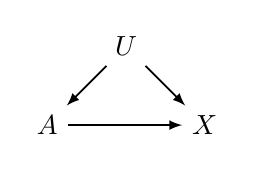
\begin{tikzpicture}[-latex ,auto ,node distance =1 cm and 2cm ,on grid ,
    semithick ,
    variable/.style ={ circle ,top color =white , 
    draw , text=blue , minimum width =1 cm},
    kernel/.style={rectangle,draw}
    ]
    \node (A)  {$A$};
    \node (U) [above right = 1cm and 1cm of A] {$U$};
    \node (X) [right = of A] {$X$};
    \draw (A) -- (X);
    \draw (U) -- (X);
    \draw (U) -- (A);
    \end{tikzpicture}

    \caption{Causal structure for the NGR regime. $U$ is an unobserved variable.}
    \label{fig:NGR}
\end{figure}

We have a dataset that allows us to estimate the distribution $P_\mu(\RV{X},\RV{A},\RV{C})$ precisely for some set of covariates $\RV{C}$. This problem is ill-posed: the covariate $\RV{C}$ does not appear in our structural assumptions. If we were to assume $\RV{C}=\RV{U}$ then we could determine the interventional distributions $P_{\mathcal{G}}(\RV{X}|do(A=a))$ via Eq. \ref{eq:trunc_fact}:
\begin{align}
    P_{\mathcal{G}}(\RV{X},\RV{C}|do(A=a)) &= P_\mu(\RV{X}|\RV{C},\RV{A}=a) P_\mu(\RV{C})\\
    P_{\mathcal{G}}(\RV{X}|do(A=a)) &= \sum_{c\in C} P_\mu(\RV{X}|\RV{C}=c,\RV{A}=a) P_\mu(\RV{C}=c) \label{eq:adjustment}
\end{align}

We will call Eq. \ref{eq:adjustment} \emph{covariate adjustment}. Observational causal inference aims to estimate causal effects by covariate adjustment. In the potential outcomes setting, the assumption of conditional ignorability is made, which entails the same estimand as in Eq. \ref{eq:adjustment} \cite{imai_covariate_2014,rubin_causal_2005,dorie_automated_2017}:
\begin{align}
    \RV{X}^{A=a} \CI \RV{A} | \RV{C} \label{eq:PO_oci}
\end{align}

In comparisons to experiments, this approach has often been criticised as yielding unreliable estimates\cite{fraker_adequacy_1987,lalonde_evaluating_1986}, though these comparisons have themselves been subject to some criticism\cite{heckman_randomization_1991}. A recent comparison with very large quantities of data and sets of covariates continued to find substantial disagreement with experimental data\cite{gordon_comparison_2018}.

A lot of analysis of observational causal inference has focussed on techniques for estimating the right hand side of equation \ref{eq:adjustment}. The consequences of the assumptions $\RV{C}=\RV{U}$ or \ref{eq:PO_oci} are less well understood. It is known that in some cases it can lead to a worse estimate of the causal effect of $\RV{A}$ on $\RV{X}$ than the a naive approach which simply assumes that $P_\mu(RV{X}|\RV{A})$ gives the appropriate causal effect. I am not aware of any work on examining whether this is likely or not.

The conditions under which covariate adjustment leads to a more biased estimate depend on a so-called ``m-strcucture.
\begin{figure}[ht]
    \centering
    \begin{tikzpicture}[-latex ,auto ,node distance =1 cm and 2cm ,on grid ,
    semithick ,
    variable/.style ={ circle ,top color =white , 
    draw , text=blue , minimum width =1 cm},
    kernel/.style={rectangle,draw}
    ]
    \node (A) {$A$};
    \node (Z) [above right = of A] {$C$};
    \node (X) [right = 4cm of A] {$X$};
    \node (A1) [right = 4cm of X] {$A$};
    \node (U1) [above right = 2cm and 1cm of A1] {$U1$};
    \node (Z1) [above right = of A1] {$C$};
    \node (U2) [above right = 1cm and 1cm of Z1] {$U2$};
    \node (X1) [right = 4cm of A1] {$X$};
    \draw (A) -- (X);
    \draw (Z) -- (X);
    \draw (Z) -- (A);
    \draw (U1) -- (Z1);
    \draw (U2) -- (Z1);
    \draw (U1) -- (A1);
    \draw (U2) -- (X1);
    \draw (A1) -- (X1);
    \end{tikzpicture}
    \caption{Two graphs $\mathcal{G}$ and $\mathcal{G}_m$, demonstrating the ``default assumption'' and an m-structure respectively}
    \label{fig:my_label}
\end{figure}


In the first case, the interventional distribution is given by Eq. \ref{eq:adjustment}, while in the second case 
\begin{align}
    P_{\mathcal{G}_m}(\RV{X}|do(A=a))&=P_\mu(\RV{X}|\RV{A}=a) \label{eq:m_structure}\\
\end{align}

Given $P_\mu(\RV{X},\RV{A},\RV{C})$, the two structures are not distinguishable on the basis of conditional independences. The distinction between the two situations can also be described using the language of potential outcomes\cite{sjolander_propensity_2009}. Under the default assumption $\mathcal{G}$, we make the assumption \ref{eq:PO_oci}, while in the second case the following assumptions are appropriate:

\begin{align}
    X^{A=a} &\not\CI A | Z \label{eq:mstruc_po3}\\
    X^{A=a} &\CI A \label{eq:mstruc_po4}
\end{align}

Proponents of the potential outcomes approach have given unclear advice on the question of whether covariate adjustment is appropriate in the second case \cite{rubin_authors_2008}\cite{noauthor_resolving_2009}. 
%!TEX root = main.tex

\subsection{Key Questions}

Key questions arising from this literature search include:

\begin{itemize}
    \item The decision rule in statistical decision problems maps observed data to a decision. However, in this setting the decision has no consequences. Causal decision theories consider which actions should be taken in light of their consequences, but observed data has no role in these theories. What is the appropriate general description of a statistical causal decision problem - that is, a problem where the objective is to select a loss-minimising decision function where decisions may have consequences.
    \item In my view, there are advantages to formulating problems in terms of consequences and losses over formulating them in terms of counterfactual effects. Is it possible to map decision rules implicit in a counterfactual effects formulation to a consequences and losses formulation in cases where the counterfactual effects can be estimated?
    \item The structural risk minimisation principle balances empirical and generalisation loss. Causal decision problems introduce the ``loss due to erroneous consequences'' which can be large even when empirical and generalisation losses are zero. Some approaches to causal discovery employ principles such as MDL that are backed by theoretical bounds on generalisation error. Is there any connection that can be made between generalisation loss and erroneous consequence loss?
    \item Given a causal inference problem in the observational setting, what is the relationship between structural intervention distance and erroneous consequence loss?
    \item Given an oracle for certain elements of a causal structure, how do loss bounds depend on which parts of the structure is revealed?
\end{itemize}

\end{document}
